\documentclass[11pt,a4paper]{article}

\usepackage[T1]{fontenc}
\usepackage[utf8]{inputenc}
\usepackage{lmodern}
\usepackage{microtype}
\usepackage[margin=2.5cm]{geometry}
\usepackage{amsmath,amssymb,bm}
\usepackage{booktabs}
\usepackage{graphicx}
\usepackage{float}
\usepackage[font=small]{caption}
\usepackage{enumitem}
\usepackage[hidelinks]{hyperref}

\setlist{itemsep=2pt,topsep=4pt}
\setlength{\parskip}{4pt}
\graphicspath{{../figures/}{../../docs/images/}}

% every number comes from ../metrics.json via make_numbers.py
% generated by make_numbers.py from ../metrics.json - do not edit
\expandafter\def\csname num@env.cpus\endcsname{2}
\expandafter\def\csname num@env.python\endcsname{3.13.16}
\expandafter\def\csname num@env.sklearn\endcsname{1.9.1}
\expandafter\def\csname num@env.numpy\endcsname{2.5.3}
\expandafter\def\csname num@A.d95\endcsname{154}
\expandafter\def\csname num@A.d50\endcsname{11}
\expandafter\def\csname num@A.d99\endcsname{331}
\expandafter\def\csname num@A.pctfeat\endcsname{19.6}
\expandafter\def\csname num@A.trainEV\endcsname{95.02}
\expandafter\def\csname num@A.testEV\endcsname{95.10}
\expandafter\def\csname num@A.testMSE\endcsname{214.7}
\expandafter\def\csname num@A.trainMSE\endcsname{217.79}
\expandafter\def\csname num@A.dropped\endcsname{217.79}
\expandafter\def\csname num@A.rmse\endcsname{14.7}
\expandafter\def\csname num@A.pcOne\endcsname{9.7}
\expandafter\def\csname num@A.pcTwo\endcsname{7.1}
\expandafter\def\csname num@B.dataMB\endcsname{188}
\expandafter\def\csname num@B.full\endcsname{3.17}
\expandafter\def\csname num@B.auto\endcsname{0.33}
\expandafter\def\csname num@B.rand\endcsname{2.69}
\expandafter\def\csname num@B.ipca\endcsname{19.1}
\expandafter\def\csname num@B.mmfitpeak\endcsname{212}
\expandafter\def\csname num@B.mmpfpeak\endcsname{24}
\expandafter\def\csname num@B.mmpfsec\endcsname{18.7}
\expandafter\def\csname num@B.fullRAM\endcsname{569}
\expandafter\def\csname num@B.randgap\endcsname{0.52}
\expandafter\def\csname num@B.ipcagap\endcsname{0.81}
\expandafter\def\csname num@B.saving\endcsname{24}
\expandafter\def\csname num@B.autosolver\endcsname{covariance\_eigh}
\expandafter\def\csname num@B.randRAM\endcsname{495}
\expandafter\def\csname num@B.autoRAM\endcsname{215}
\expandafter\def\csname num@C.gamma\endcsname{0.0411}
\expandafter\def\csname num@C.kernel\endcsname{rbf}
\expandafter\def\csname num@C.cv\endcsname{96.1}
\expandafter\def\csname num@C.testsup\endcsname{96.4}
\expandafter\def\csname num@C.testunsup\endcsname{73.6}
\expandafter\def\csname num@C.raw\endcsname{64.8}
\expandafter\def\csname num@C.linear\endcsname{75.2}
\expandafter\def\csname num@C.pregamma\endcsname{0.0478}
\expandafter\def\csname num@C.prekernel\endcsname{sigmoid}
\expandafter\def\csname num@C.premse\endcsname{21.76}
\expandafter\def\csname num@C.cvstd\endcsname{1.0}
\expandafter\def\csname num@C.nwithin\endcsname{7}
\expandafter\def\csname num@C.book\endcsname{32.7863}
\expandafter\def\csname num@C.nsettings\endcsname{20}
\expandafter\def\csname num@C.lle\endcsname{98.2}
\expandafter\def\csname num@C.isomap\endcsname{99.2}
\expandafter\def\csname num@C.tsne\endcsname{98.7}
\expandafter\def\csname num@C.mds\endcsname{75.1}
\expandafter\def\csname num@C.pca\endcsname{71.6}
\expandafter\def\csname num@C.lleCorr\endcsname{0.997}
\expandafter\def\csname num@D.n\endcsname{5{,}000}
\expandafter\def\csname num@D.tsne\endcsname{93.3}
\expandafter\def\csname num@D.tsneraw\endcsname{92.9}
\expandafter\def\csname num@D.pca\endcsname{41.4}
\expandafter\def\csname num@D.tsnesec\endcsname{16.5}
\expandafter\def\csname num@D.tsnerawsec\endcsname{16.7}
\expandafter\def\csname num@D.lle\endcsname{68.2}
\expandafter\def\csname num@D.isomap\endcsname{50.4}
\expandafter\def\csname num@D.mds\endcsname{45.3}
\expandafter\def\csname num@D.kpca\endcsname{40.7}
\expandafter\def\csname num@D.mdssec\endcsname{191}
\expandafter\def\csname num@E.svmraw\endcsname{97.01}
\expandafter\def\csname num@E.svmpca\endcsname{97.48}
\expandafter\def\csname num@E.svmfit\endcsname{2.6}
\expandafter\def\csname num@E.svmpred\endcsname{2.7}
\expandafter\def\csname num@E.svmn\endcsname{20{,}000}
\expandafter\def\csname num@E.svmd\endcsname{154}
\expandafter\def\csname num@E.svmrawMB\endcsname{39.3}
\expandafter\def\csname num@E.svmpcaMB\endcsname{8.6}
\expandafter\def\csname num@E.rfraw\endcsname{97.05}
\expandafter\def\csname num@E.rfpca\endcsname{94.95}
\expandafter\def\csname num@E.rffit\endcsname{0.41}
\expandafter\def\csname num@E.rfrawsec\endcsname{29.8}
\expandafter\def\csname num@E.rfrawMB\endcsname{146}
\expandafter\def\csname num@E.rfpcaMB\endcsname{213}
\expandafter\def\csname num@E.rfpcasec\endcsname{72.1}
\expandafter\def\csname num@E.smraw\endcsname{92.64}
\expandafter\def\csname num@E.smpca\endcsname{92.32}
\expandafter\def\csname num@E.smfit\endcsname{8.3}
\expandafter\def\csname num@E.svmdiff\endcsname{$+$0.47}
\expandafter\def\csname num@E.svmdifflo\endcsname{$+$0.31}
\expandafter\def\csname num@E.svmdiffhi\endcsname{$+$0.63}
\expandafter\def\csname num@E.rfdiff\endcsname{$-$2.10}
\expandafter\def\csname num@E.rfdifflo\endcsname{$-$2.46}
\expandafter\def\csname num@E.rfdiffhi\endcsname{$-$1.74}
\expandafter\def\csname num@E.smdiff\endcsname{$-$0.32}
\expandafter\def\csname num@E.smdifflo\endcsname{$-$0.61}
\expandafter\def\csname num@E.smdiffhi\endcsname{$-$0.03}
\expandafter\def\csname num@E.same\endcsname{97.13}
\expandafter\def\csname num@E.samediff\endcsname{$+$0.12}
\expandafter\def\csname num@E.samedifflo\endcsname{$+$0.01}
\expandafter\def\csname num@E.samediffhi\endcsname{$+$0.23}
\expandafter\def\csname num@E.repeats\endcsname{3}
\expandafter\def\csname num@E.svmgain\endcsname{0.47}
\expandafter\def\csname num@E.samegain\endcsname{0.12}
\expandafter\def\csname num@D.knn784\endcsname{92.8}
\expandafter\def\csname num@D.knn784std\endcsname{0.7}
\expandafter\def\csname num@F.falo\endcsname{2.99}
\expandafter\def\csname num@F.fahi\endcsname{3.69}
\expandafter\def\csname num@F.d\endcsname{154}
\expandafter\def\csname num@F.thr\endcsname{427}
\expandafter\def\csname num@F.trainthr\endcsname{420}
\expandafter\def\csname num@F.fa\endcsname{3.34}
\expandafter\def\csname num@F.fatrain\endcsname{3.66}
\expandafter\def\csname num@F.mean\endcsname{65.0}
\expandafter\def\csname num@F.auc\endcsname{0.791}
\expandafter\def\csname num@F.rotated\endcsname{12.7}
\expandafter\def\csname num@F.mirrored\endcsname{17.2}
\expandafter\def\csname num@F.shifted\endcsname{90.2}
\expandafter\def\csname num@F.dimmed\endcsname{0.0}
\expandafter\def\csname num@F.errflag\endcsname{6.0}
\expandafter\def\csname num@F.errunflag\endcsname{2.4}
\expandafter\def\csname num@F.nflag\endcsname{334}
\expandafter\def\csname num@F.nerrflag\endcsname{20}
\expandafter\def\csname num@F.nerr\endcsname{252}
\expandafter\def\csname num@F.bestvarAUC\endcsname{0.819}
\expandafter\def\csname num@F.bestvar\endcsname{80}
\expandafter\def\csname num@F.bestvard\endcsname{44}

% generated by make_numbers.py from ../metrics.json - do not edit
\newcommand{\TableVariance}{
\begin{tabular}{rrrrrr}
\toprule
target & $d$ & features & train var. & test var. & test RMSE \\
\midrule
50\% & 11 & 1.4\% & 50.92\% & 51.55\% & 46.1 \\
80\% & 44 & 5.6\% & 80.33\% & 80.87\% & 29.0 \\
90\% & 87 & 11.1\% & 90.01\% & 90.27\% & 20.7 \\
95\% & 154 & 19.6\% & 95.02\% & 95.10\% & 14.7 \\
99\% & 331 & 42.2\% & 99.00\% & 99.02\% & 6.6 \\
\bottomrule
\end{tabular}}
\newcommand{\TableStorage}{
\begin{tabular}{lrrr}
\toprule
representation & bytes/image & vs float32 pixels & vs uint8 pixels \\
\midrule
raw pixels, uint8 (as shipped) & 784 & 25.0\% & 100.0\% \\
raw pixels, float32 & 3{,}136 & 100.0\% & 400.0\% \\
PCA codes, float32 (154 values) & 616 & 19.6\% & 78.6\% \\
PCA codes, float16 (154 values) & 308 & 9.8\% & 39.3\% \\
\bottomrule
\end{tabular}}
\newcommand{\TableSolvers}{
\begin{tabular}{llrrrr}
\toprule
solver & data in & fit (s) & RAM (MB) & variance & $\Delta$ test MSE \\
\midrule
PCA, full SVD & RAM & 3.17 & 569 & 0.9502 & $+$0.00\% \\
PCA, solver=\textquotesingle{}auto\textquotesingle{} & RAM & 0.33 & 215 & 0.9502 & $-$0.00\% \\
Randomized PCA & RAM & 2.69 & 495 & 0.9498 & $+$0.52\% \\
Incremental PCA, partial\_fit & RAM & 19.08 & 212 & 0.9495 & $+$0.81\% \\
Incremental PCA, memmap + fit() & disk & 19.24 & 212 & 0.9495 & $+$0.81\% \\
Incremental PCA, memmap + partial\_fit & disk & 18.75 & 24 & 0.9495 & $+$0.81\% \\
\bottomrule
\end{tabular}}
\newcommand{\TableManifold}{
\begin{tabular}{lrrr}
\toprule
method & time (s) & downstream accuracy & $\max_j |\mathrm{corr}(z_j, t)|$ \\
\midrule
PCA & $<$0.01 & 71.6\% & 0.219 \\
Kernel PCA (rbf) & 0.09 & 96.4\% & 0.461 \\
LLE & 0.07 & 98.2\% & 0.997 \\
Isomap & 0.15 & 99.2\% & 0.992 \\
MDS & 1.90 & 75.1\% & 0.179 \\
t-SNE & 2.32 & 98.7\% & 0.904 \\
\bottomrule
\end{tabular}}
\newcommand{\TableMaps}{
\begin{tabular}{lrr}
\toprule
method & time (s) & kNN accuracy ($\pm$ std over folds) \\
\midrule
PCA & 0.2 & 41.4\% $\pm$ 1.4 \\
Kernel PCA & 1.3 & 40.7\% $\pm$ 1.9 \\
LLE & 5.3 & 68.2\% $\pm$ 1.2 \\
Isomap & 5.9 & 50.4\% $\pm$ 1.6 \\
MDS & 190.5 & 45.3\% $\pm$ 0.8 \\
t-SNE & 16.5 & 93.3\% $\pm$ 0.9 \\
t-SNE (raw pixels) & 16.7 & 92.9\% $\pm$ 0.8 \\
\emph{no reduction: all 784 pixels} & -- & 92.8\% $\pm$ 0.7 \\
\bottomrule
\end{tabular}}
\newcommand{\TableClassifiers}{
\begin{tabular}{llrrrrr}
\toprule
classifier & features & train & fit (s) & predict (s) & accuracy (95\% CI) & MB \\
\midrule
Softmax Regression & 784 pixels & 60{,}000 & 34.1 & 0.01 & 92.64 (92.13--93.15) & 0.0 \\
Softmax Regression & PCA (154) & 60{,}000 & 4.1 & 0.04 & 92.32 (91.80--92.84) & 0.5 \\
Random Forest & 784 pixels & 60{,}000 & 29.8 & 0.27 & 97.05 (96.72--97.38) & 146.1 \\
Random Forest & PCA (154) & 60{,}000 & 72.1 & 0.24 & 94.95 (94.52--95.38) & 212.8 \\
SVM & 784 pixels & 20{,}000 & 22.9 & 26.21 & 97.01 (96.68--97.34) & 39.3 \\
SVM & PCA (154) & 20{,}000 & 8.7 & 9.88 & 97.48 (97.17--97.79) & 8.6 \\
SVM & PCA, raw $\gamma$ (154) & 20{,}000 & 7.6 & 9.07 & 97.13 (96.80--97.46) & 8.2 \\
\bottomrule
\end{tabular}}
\newcommand{\TableDetector}{
\begin{tabular}{lrr}
\toprule
input (10{,}000 test images) & flagged & median error \\
\midrule
clean test digits & 3.3\% & 198 \\
noise & 100.0\% & 10{,}908 \\
inverted & 100.0\% & 26{,}459 \\
shuffled & 100.0\% & 5{,}297 \\
rotated & 12.7\% & 246 \\
mirrored & 17.2\% & 269 \\
shifted & 90.2\% & 1{,}119 \\
gaussian & 100.0\% & 2{,}231 \\
dimmed & 0.0\% & 18 \\
\bottomrule
\end{tabular}}
\newcommand{\TableVarSweep}{
\begin{tabular}{rrrrr}
\toprule
variance & $d$ & false alarms & mean detection & ROC-AUC \\
\midrule
80\% & 44 & 2.84\% & 67.0\% & 0.819 \\
90\% & 87 & 3.12\% & 66.3\% & 0.806 \\
95\% & 154 & 3.34\% & 65.0\% & 0.791 \\
99\% & 331 & 3.67\% & 65.5\% & 0.786 \\
\bottomrule
\end{tabular}}

\newcommand{\R}[1]{\csname num@#1\endcsname}

\newcommand{\x}{\mathbf{x}}
\newcommand{\X}{\mathbf{X}}
\newcommand{\w}{\mathbf{w}}
\newcommand{\W}{\mathbf{W}}
\newcommand{\z}{\mathbf{z}}
\newcommand{\bmu}{\boldsymbol{\mu}}
\newcommand{\T}{^{\top}}
\DeclareMathOperator{\tr}{tr}

\title{Dimensionality Reduction for High-Dimensional Data:\\ PCA, Kernel PCA and t-SNE on MNIST, from Notebook to Monitored Service}
\author{Xaysomvang (Tom) Thammavong\\[2pt]
\small \url{https://github.com/ToMooGo/dimensionality-reduction-mlops}}
\date{October 2026}

\begin{document}
\maketitle

\begin{abstract}
\noindent
This report documents an end-to-end project on dimensionality reduction. The methods are those of Géron, \emph{Hands-On Machine Learning with Scikit-Learn, Keras and TensorFlow} (2nd ed.), Chapter~8. They are applied to the 70{,}000 MNIST digits.
Principal Component Analysis keeps \R{A.trainEV}\% of the training variance with \R{A.d95} of 784 components. The decompressed test images keep \R{A.testEV}\% of the test variance.
Incremental PCA fed from a memory-mapped file needs at most \R{B.mmpfpeak}~MB of memory, against \R{B.fullRAM}~MB for a full SVD with the data in RAM. Calling \texttt{fit()} on the memory map, as the book does, copies the whole array into memory.
Kernel PCA is tuned over \R{C.nsettings} kernel and $\gamma$ settings, with two selection rules. The supervised rule reaches \R{C.testsup}\% held-out accuracy on the Swiss roll. The unsupervised rule (lowest pre-image error) chooses a different kernel, which reaches only \R{C.testunsup}\%.
t-SNE separates the digits far better than PCA, Kernel PCA, LLE, Isomap or MDS: \R{D.tsne}\% $k$-nearest-neighbour accuracy in 2D, against \R{D.pca}\% for PCA and \R{D.knn784}\% for the same classifier on all 784 pixels.
With PCA features, an RBF-kernel SVM trains \R{E.svmfit} times and predicts \R{E.svmpred} times faster, and its accuracy rises from \R{E.svmraw}\% to \R{E.svmpca}\%. An ablation shows that most of this gain comes from the kernel width that the default \texttt{gamma} implies on the new features, not from the compression itself. A Random Forest instead becomes slower and less accurate.
Finally, the PCA reconstruction error flags unusual inputs at \R{F.fa}\% false alarms.
Everything runs as one Prefect pipeline with MLflow tracking, a model registry with quality gates, a FastAPI service and PostgreSQL monitoring, started by \texttt{docker compose up}.
\end{abstract}

\tableofcontents
\newpage

%=====================================================================================
\section{Introduction}

MNIST images have 784 pixels, but handwritten digits occupy a tiny part of that space. They are made of connected strokes on a white background, roughly centred. Chapter~8 of Géron's book calls this the \emph{manifold assumption}: most real high-dimensional data lie close to a much lower-dimensional manifold. Dimensionality reduction exploits it for three purposes: to compress data, to speed up the algorithms that come after it, and to visualise data in two dimensions.

The project asks six questions, labelled A--F throughout the repository:
\begin{enumerate}[label=\Alph*.]
\item How many principal components keep 95\% of MNIST's variance, and how good are the decompressed images?
\item Can PCA run on data that does not fit in memory, and do the faster solvers give the same answer?
\item How should Kernel PCA be tuned when there is no obvious performance measure?
\item Which 2D map of MNIST best separates the digits?
\item Does training on compressed features make classifiers faster, and at what cost in accuracy?
\item Can the reconstruction error of PCA flag inputs that do not look like digits?
\end{enumerate}
Each question is answered with the book's method, measured on held-out data, and reported with its limits. The models answering A, E and F are deployed behind a web service, together with the maps from D. Sections~\ref{sec:pca}--\ref{sec:detector} derive the mathematics and present the results. Section~\ref{sec:system} describes the system.

%=====================================================================================
\section{Data and evaluation protocol}\label{sec:data}

MNIST is loaded as in the book with \texttt{fetch\_openml("mnist\_784")}: 70{,}000 images of $28\times 28$ pixels with intensities from 0 (background) to 255 (ink). Following the book (exercise~9), the first 60{,}000 images form the training set and the last 10{,}000 the test set. When OpenML cannot be reached, the original MNIST files are downloaded from a mirror instead. They are accepted only if their MD5 checksums match the official ones, and they give the same matrix in the same order.

All randomness is seeded. Every model is fitted on training data only, and every quality figure is measured on the test set unless stated otherwise. Timings are wall-clock seconds on a \R{env.cpus}-CPU machine (Python \R{env.python}, scikit-learn \R{env.sklearn}, NumPy \R{env.numpy}). They are medians of three runs; fits slower than 30~s (Section~\ref{sec:scaling}) or 60~s (Section~\ref{sec:classify}) are timed once. They compare methods on the same machine and are not absolute benchmarks.

A test-set number is a point estimate. Following the book (Chapter~2, p.~83), its precision is given by a 95\% confidence interval computed with \texttt{scipy.stats.t.interval} from the per-image values. For an accuracy the per-image value is 1 for a correct prediction and 0 otherwise. For the difference between two models evaluated on the same images it is the per-image difference of those values, which gives a \emph{paired} interval.

%=====================================================================================
\section{Principal Component Analysis}\label{sec:pca}

Let $\x^{(1)},\dots,\x^{(m)}\in\mathbb{R}^n$ be the training images ($m=60{,}000$, $n=784$). Let
\begin{equation}
\bmu=\frac{1}{m}\sum_{i=1}^{m}\x^{(i)}, \qquad
\mathbf{S}=\frac{1}{m-1}\sum_{i=1}^{m}\big(\x^{(i)}-\bmu\big)\big(\x^{(i)}-\bmu\big)\T
\end{equation}
be their mean and sample covariance matrix. $\X_c$ denotes the $m\times n$ matrix of centred images, so that $\mathbf{S}=\X_c\T\X_c/(m-1)$.

\subsection{Preserving the variance}

PCA looks for the unit vector $\mathbf{c}_1$ along which the projected data vary most. The projection of a centred image on $\mathbf{c}$ is $\mathbf{c}\T(\x^{(i)}-\bmu)$, and its sample variance is
\begin{equation}
\frac{1}{m-1}\sum_{i=1}^{m}\big(\mathbf{c}\T(\x^{(i)}-\bmu)\big)^2
=\frac{1}{m-1}\sum_{i=1}^{m}\mathbf{c}\T(\x^{(i)}-\bmu)(\x^{(i)}-\bmu)\T\mathbf{c}
=\mathbf{c}\T\mathbf{S}\,\mathbf{c}.
\end{equation}
We maximise $\mathbf{c}\T\mathbf{S}\mathbf{c}$ subject to $\mathbf{c}\T\mathbf{c}=1$ with a Lagrange multiplier $\lambda$:
\begin{align}
\mathcal{L}(\mathbf{c},\lambda)&=\mathbf{c}\T\mathbf{S}\,\mathbf{c}-\lambda\,(\mathbf{c}\T\mathbf{c}-1),\\
\frac{\partial\mathcal{L}}{\partial\mathbf{c}}&=2\mathbf{S}\,\mathbf{c}-2\lambda\,\mathbf{c}=\mathbf{0}
\quad\Longrightarrow\quad \mathbf{S}\,\mathbf{c}=\lambda\,\mathbf{c}.
\end{align}
So $\mathbf{c}$ must be an eigenvector of $\mathbf{S}$. Its variance is then $\mathbf{c}\T\mathbf{S}\mathbf{c}=\lambda\,\mathbf{c}\T\mathbf{c}=\lambda$, so the maximum is reached by the eigenvector with the largest eigenvalue $\lambda_1$. The second component maximises the same quantity under the extra constraint $\mathbf{c}_2\T\mathbf{c}_1=0$. Adding a multiplier $\phi$ for it gives $2\mathbf{S}\mathbf{c}_2-2\lambda\mathbf{c}_2-\phi\,\mathbf{c}_1=\mathbf{0}$. Multiplying on the left by $\mathbf{c}_1\T$ and using $\mathbf{c}_1\T\mathbf{S}=\lambda_1\mathbf{c}_1\T$ and $\mathbf{c}_1\T\mathbf{c}_2=0$ gives $\phi=0$. Hence $\mathbf{c}_2$ is the eigenvector with the second largest eigenvalue, and so on. Because $\mathbf{S}$ is symmetric, its eigenvectors are orthonormal and its eigenvalues $\lambda_1\ge\lambda_2\ge\dots\ge\lambda_n\ge 0$ are real.

\subsection{The same axes minimise the reconstruction error}

The book gives a second justification: the chosen axes also minimise the mean squared distance between the data and their projection. Let $\W_d=[\mathbf{c}_1,\dots,\mathbf{c}_d]$ have orthonormal columns ($\W_d\T\W_d=\mathbf{I}_d$), and write $\mathbf{u}=\x-\bmu$. The projection onto the subspace is $\W_d\W_d\T\mathbf{u}$, and the squared residual is
\begin{align}
\big\|\mathbf{u}-\W_d\W_d\T\mathbf{u}\big\|^2
&=\mathbf{u}\T\mathbf{u}-2\,\mathbf{u}\T\W_d\W_d\T\mathbf{u}+\mathbf{u}\T\W_d\underbrace{\W_d\T\W_d}_{\mathbf{I}_d}\W_d\T\mathbf{u}\nonumber\\
&=\|\mathbf{u}\|^2-\|\W_d\T\mathbf{u}\|^2 .
\end{align}
Summing over the training set and dividing by $m-1$,
\begin{equation}
\frac{1}{m-1}\sum_{i=1}^{m}\big\|\mathbf{u}^{(i)}-\W_d\W_d\T\mathbf{u}^{(i)}\big\|^2=\tr(\mathbf{S})-\tr\!\big(\W_d\T\mathbf{S}\,\W_d\big).
\end{equation}
$\tr(\mathbf{S})$ does not depend on $\W_d$. Minimising the residual is therefore the same as maximising the projected variance $\tr(\W_d\T\mathbf{S}\W_d)$, and the first $d$ eigenvectors do both.

\subsection{Computing the components with the SVD}

The book computes PCA with the singular value decomposition $\X_c=\mathbf{U}\bm{\Sigma}\mathbf{V}\T$ (Equation~8-1). Then
\begin{equation}
\mathbf{S}=\frac{\X_c\T\X_c}{m-1}=\frac{\mathbf{V}\bm{\Sigma}\mathbf{U}\T\mathbf{U}\bm{\Sigma}\mathbf{V}\T}{m-1}=\mathbf{V}\,\frac{\bm{\Sigma}^2}{m-1}\,\mathbf{V}\T ,
\end{equation}
because $\mathbf{U}\T\mathbf{U}=\mathbf{I}$. This is an eigendecomposition of $\mathbf{S}$. The columns of $\mathbf{V}$ are the principal components, and the eigenvalues are $\lambda_j=\sigma_j^2/(m-1)$. The \emph{explained variance ratio} of component $j$ is $\lambda_j/\sum_k\lambda_k$. The first notebook checks that the book's NumPy code and scikit-learn find the same first two components up to sign; the cosine between them is 1 to six decimals. The first two components explain \R{A.pcOne}\% and \R{A.pcTwo}\% of the variance.

\subsection{Projection, decompression and the reconstruction error}

Compression projects a centred image onto the first $d$ components (Equation~8-2). Decompression maps the code back (Equation~8-3):
\begin{equation}
\z=\W_d\T(\x-\bmu)\in\mathbb{R}^d,\qquad \hat{\x}=\W_d\,\z+\bmu .
\end{equation}
The book defines the reconstruction error as the mean squared distance between $\x$ and $\hat{\x}$. Its value on the training set follows from the derivation above. Write $\x^{(i)}-\bmu=\sum_{j=1}^{n}a_{ij}\mathbf{c}_j$ in the eigenbasis. Then $\x^{(i)}-\hat{\x}^{(i)}=\sum_{j>d}a_{ij}\mathbf{c}_j$, and by orthonormality $\|\x^{(i)}-\hat{\x}^{(i)}\|^2=\sum_{j>d}a_{ij}^2$. Averaging over images and pixels,
\begin{equation}
\mathrm{MSE}_{\text{train}}=\frac{1}{mn}\sum_{i=1}^{m}\sum_{j>d}a_{ij}^2
=\frac{1}{mn}\sum_{j>d}(m-1)\lambda_j
=\frac{m-1}{m}\cdot\frac{1}{n}\sum_{j>d}\lambda_j ,
\label{eq:mse-dropped}
\end{equation}
where we used $\sum_i a_{ij}^2=(m-1)\lambda_j$, since $a_{ij}$ is the centred coordinate along $\mathbf{c}_j$. \emph{The training reconstruction error is the variance of the dropped components per pixel.} The pipeline checks this identity on every run. At $d=\R{A.d95}$ both sides equal \R{A.trainMSE}.

\subsection{Choosing the number of dimensions}

The book's rule picks the smallest $d$ whose cumulative explained variance reaches 95\%. On MNIST this gives $d=\R{A.d95}$, \R{A.pctfeat}\% of the 784 features, which is the book's ``just over 150''. \texttt{PCA(n\_components=0.95)} returns the same $d$. Figure~\ref{fig:variance} shows the curve, and Table~\ref{tab:variance} gives several compression levels. The test set keeps slightly \emph{more} of its variance than the training set (\R{A.testEV}\% vs \R{A.trainEV}\% at 95\%), so the compression generalises. The typical error of a test pixel is \R{A.rmse} grey levels out of 255, and Figure~\ref{fig:recon} shows that the digits remain clearly legible.

\begin{figure}[H]
\centering
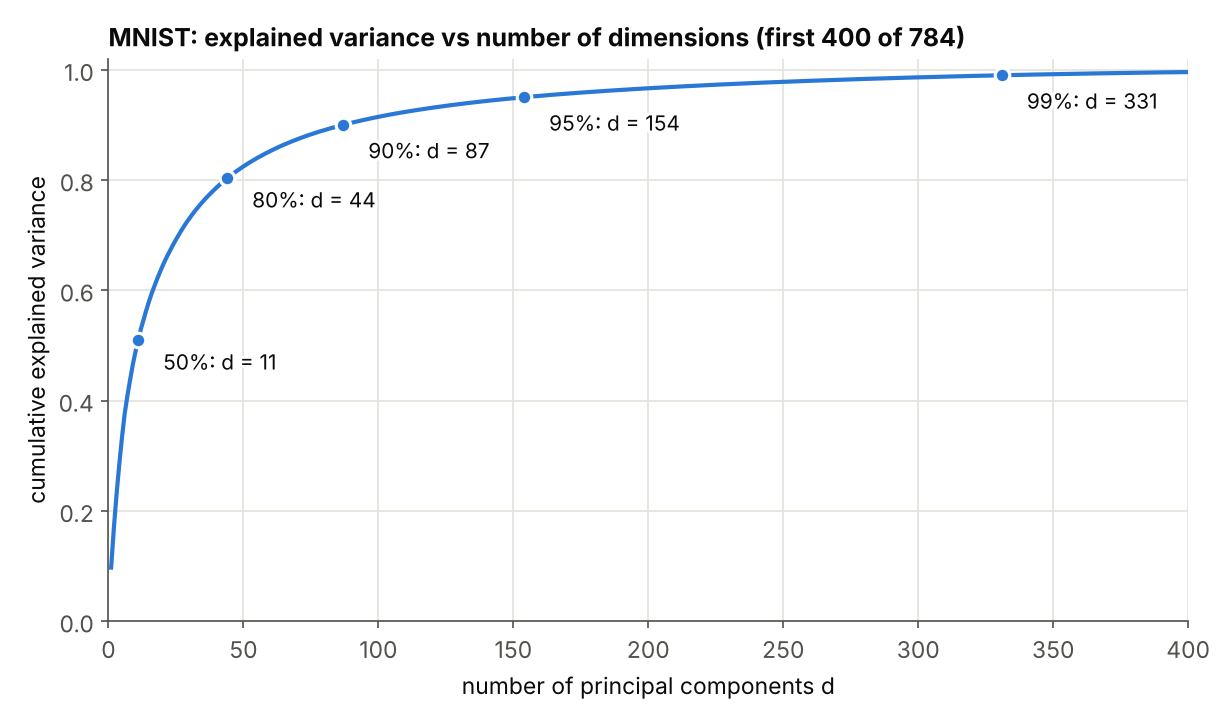
\includegraphics[width=0.72\textwidth]{a_explained_variance.png}
\caption{Cumulative explained variance of MNIST's principal components, with the number of components needed for 50\%, 80\%, 90\%, 95\% and 99\% of the variance.}
\label{fig:variance}
\end{figure}

\begin{table}[H]
\centering
\caption{Compression levels. ``Test variance'' is the share of the test set's variance that survives compression followed by decompression; RMSE is in grey levels (0--255).}
\label{tab:variance}
\small\TableVariance
\end{table}

\begin{figure}[H]
\centering
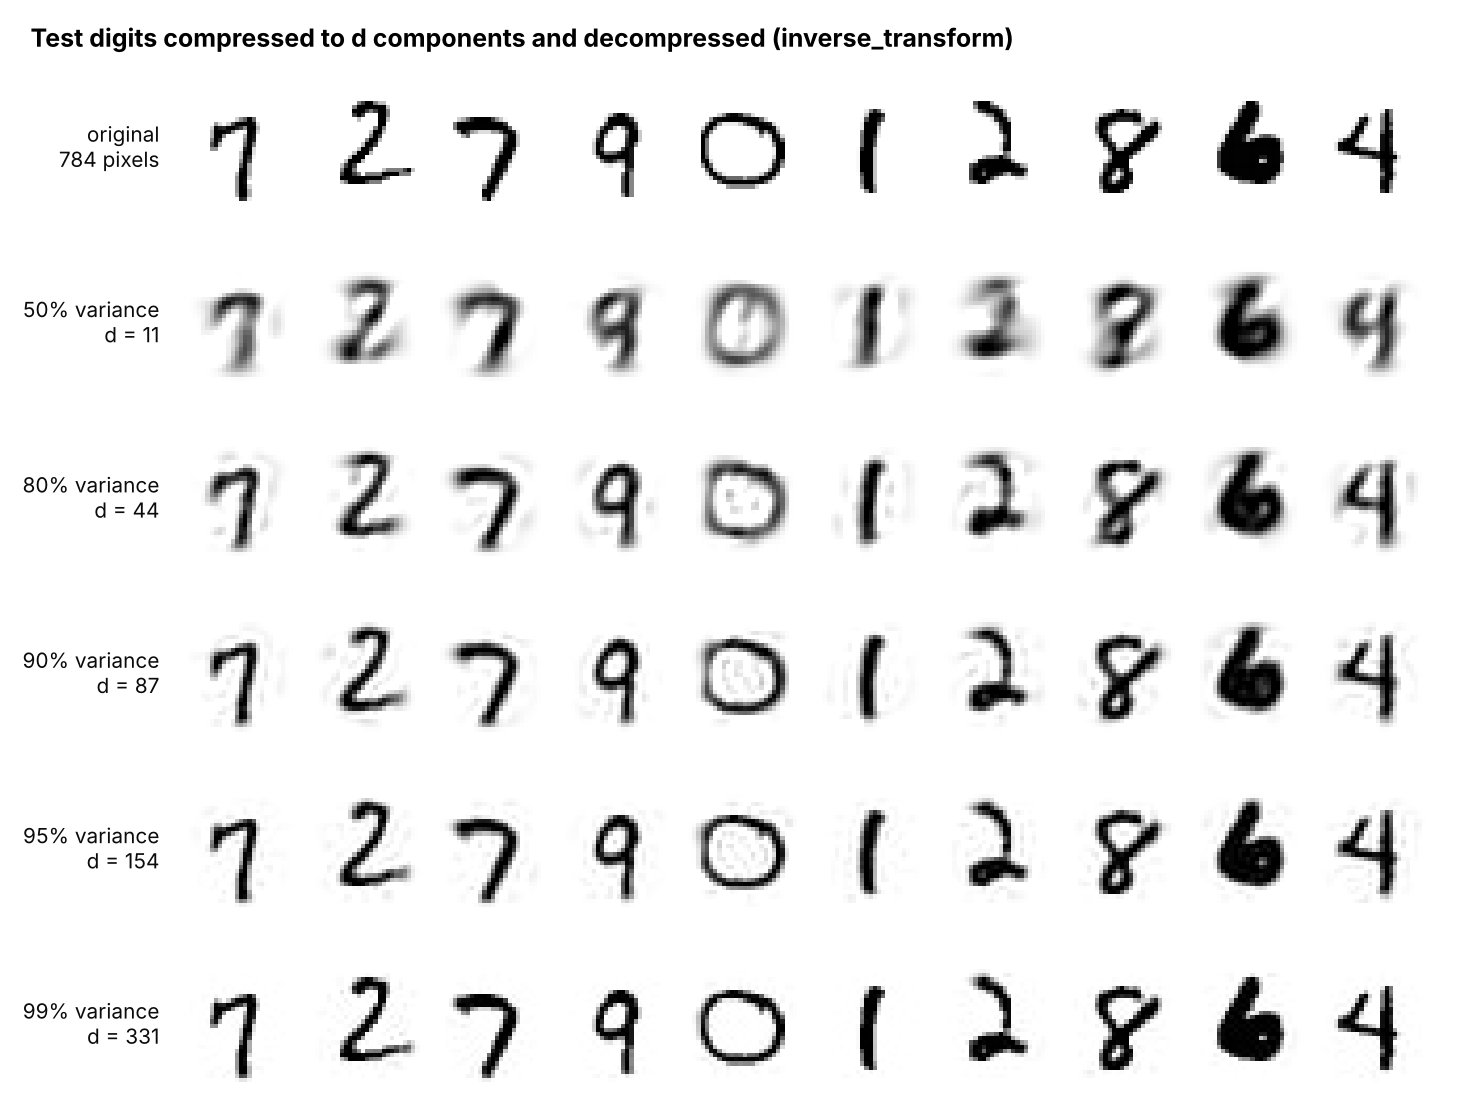
\includegraphics[width=0.8\textwidth]{a_reconstructions.png}
\caption{Ten test digits, compressed to $d$ components and decompressed.}
\label{fig:recon}
\end{figure}

\subsection{``Less than 20\% of its original size'': features or bytes?}

The book's figure compares numbers of features: $154/784=19.6\%$. MNIST, however, is stored with one byte per pixel, while PCA codes are floating-point numbers. Table~\ref{tab:storage} shows that float32 codes take 78.6\% of the bytes of the original uint8 file, and float16 codes 39.3\%. The saving in memory depends on how both sides are stored.

\begin{table}[H]
\centering
\caption{Storage per image for the raw pixels and for the 154-value PCA codes.}
\label{tab:storage}
\small\TableStorage
\end{table}

%=====================================================================================
\section{PCA at scale}\label{sec:scaling}

\subsection{Solvers and their cost}

The book compares the full SVD, with cost $O(mn^2)+O(n^3)$, and Randomized PCA, which approximates the first $d$ components in $O(md^2)+O(d^3)$. Both need the whole training matrix in memory. In practice each pass of the randomized algorithm also multiplies the $m\times n$ data by an $n\times(d+p)$ block, which costs $O(mnd)$. With $d/n=154/784\approx0.2$ the saving over the exact methods is therefore small on MNIST. Since version~1.5, scikit-learn's \texttt{svd\_solver="auto"} also considers a third route for tall data ($m\gg n$). It forms the $n\times n$ covariance matrix in $O(mn^2)$ and eigendecomposes it in $O(n^3)$, which is exactly the eigenproblem of Section~\ref{sec:pca}. On MNIST, \texttt{"auto"} picked \texttt{\R{B.autosolver}}.

\subsection{Incremental PCA}

Incremental PCA processes mini-batches one at a time, so the full matrix never has to be in memory. The idea can be seen in the statistics it must keep up to date. Suppose batch $A$ ($n_A$ images, mean $\bmu_A$, scatter matrix $\mathbf{M}_A=\sum_{i\in A}(\x^{(i)}-\bmu_A)(\x^{(i)}-\bmu_A)\T$) has been processed, and batch $B$ arrives. The combined mean is
\begin{equation}
\bmu_{AB}=\frac{n_A\bmu_A+n_B\bmu_B}{n_A+n_B}.
\end{equation}
For the combined scatter, write $\x-\bmu_{AB}=(\x-\bmu_A)+(\bmu_A-\bmu_{AB})$ for $\x\in A$. The cross terms vanish because $\sum_{i\in A}(\x^{(i)}-\bmu_A)=\mathbf{0}$, so
\begin{equation}
\sum_{i\in A}(\x^{(i)}-\bmu_{AB})(\x^{(i)}-\bmu_{AB})\T=\mathbf{M}_A+n_A(\bmu_A-\bmu_{AB})(\bmu_A-\bmu_{AB})\T ,
\end{equation}
and similarly for $B$. Using $\bmu_A-\bmu_{AB}=\frac{n_B}{n_A+n_B}(\bmu_A-\bmu_B)$ and $\bmu_B-\bmu_{AB}=-\frac{n_A}{n_A+n_B}(\bmu_A-\bmu_B)$, the two correction terms add up to
\begin{equation}
\mathbf{M}_{AB}=\mathbf{M}_A+\mathbf{M}_B+\frac{n_A n_B}{n_A+n_B}\,(\bmu_A-\bmu_B)(\bmu_A-\bmu_B)\T .
\end{equation}
The combined statistics therefore depend only on the summaries of each batch, not on the images themselves. scikit-learn's \texttt{IncrementalPCA} (the algorithm of Ross et~al.\ cited by the book) keeps a rank-$d$ SVD summary instead of the full $n\times n$ matrix and applies the same mean correction. This is why its result differs slightly from the exact components.

\subsection{Out-of-core training with a memory map}

The book stores the data in a binary file, opens it with \texttt{np.memmap} and passes the memory map \texttt{X\_mm} to the \texttt{fit()} method of an \texttt{IncrementalPCA} with 154 components. Measuring the peak memory of that call gives \R{B.mmfitpeak}~MB. The measure is the peak of the heap allocations that NumPy reports to Python's \texttt{tracemalloc}. It does not count pages of the memory-mapped file, which the operating system can drop at any time, or the BLAS library's own small internal buffers. That is the whole \R{B.dataMB}~MB training matrix. The reason is that \texttt{fit()} first validates its input with \texttt{copy=True}, which copies the memory map into RAM. Calling \texttt{partial\_fit} on one slice of the memory map at a time keeps the peak at \R{B.mmpfpeak}~MB and gives identical components. This is \R{B.saving} times less memory than a full SVD with the data in RAM (\R{B.fullRAM}~MB).

\subsection{Results}

Table~\ref{tab:solvers} and Figure~\ref{fig:solvers} summarise the six variants. All of them find essentially the same subspace: the test reconstruction error of Randomized PCA is \R{B.randgap}\% above the exact SVD, and that of Incremental PCA \R{B.ipcagap}\%. Randomized PCA is not dramatically faster here (\R{B.rand}~s vs \R{B.full}~s), because with only $n=784$ features the full SVD is already cheap. The book's complexity argument pays off when $n$ is large. The covariance route chosen by \texttt{"auto"} is the fastest (\R{B.auto}~s) and needs little memory beyond the data. Incremental PCA is the slowest solver (\R{B.ipca}~s), and the price of the out-of-core version is time, not accuracy.

\begin{table}[H]
\centering
\caption{154 components of the 60{,}000 training images. RAM = peak allocations while fitting, plus the training matrix when it is held in memory. $\Delta$ test MSE is relative to the exact SVD.}
\label{tab:solvers}
\small\TableSolvers
\end{table}

\begin{figure}[H]
\centering
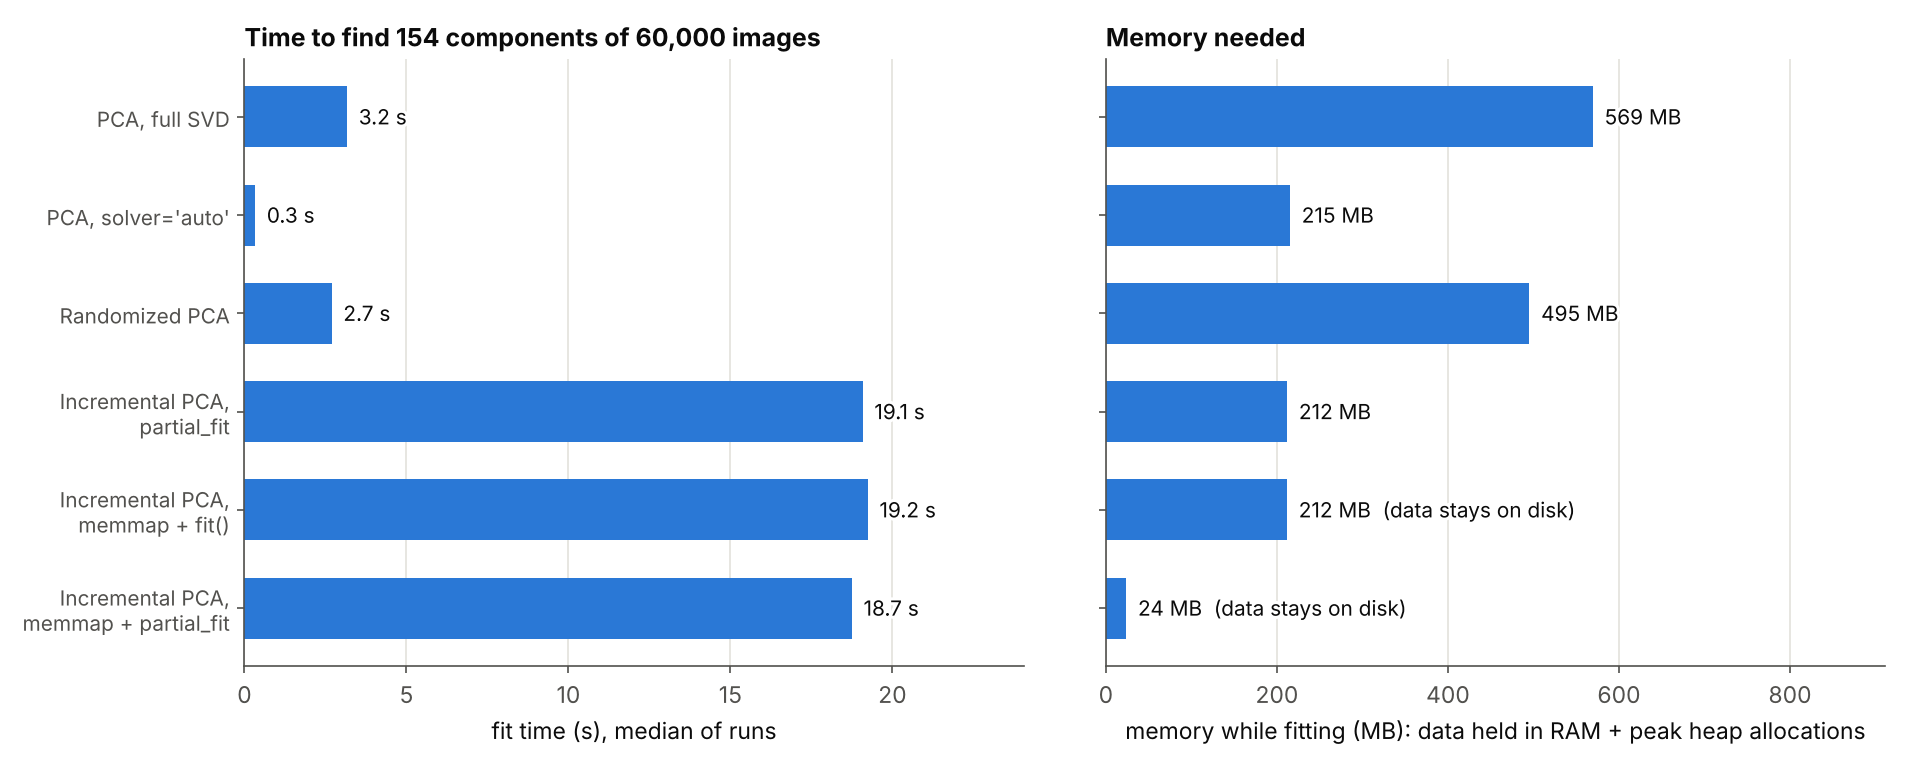
\includegraphics[width=\textwidth]{b_solvers.png}
\caption{Fit time and memory of the six PCA variants.}
\label{fig:solvers}
\end{figure}

\begin{figure}[H]
\centering
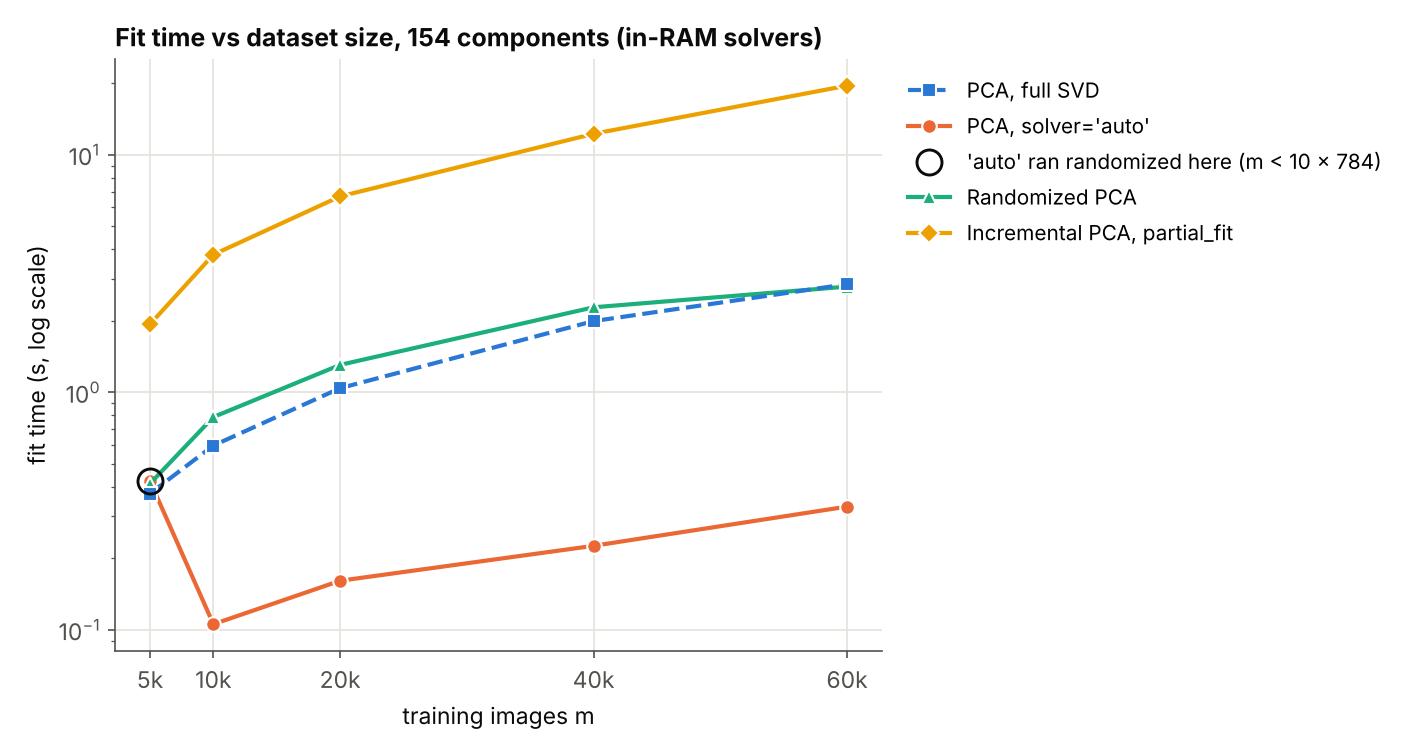
\includegraphics[width=0.7\textwidth]{b_timing_curve.png}
\caption{Fit time against the number of training images (log scale).}
\label{fig:timing}
\end{figure}

%=====================================================================================
\section{Kernel PCA}\label{sec:kpca}

\subsection{PCA in a feature space}

Kernel PCA applies PCA after an implicit map $\phi:\mathbb{R}^n\to\mathcal{F}$ into a high-dimensional feature space. Only inner products $k(\x,\x')=\phi(\x)\T\phi(\x')$ are computed: this is the kernel trick of Chapter~5. The kernels used here are the RBF kernel $k(\x,\x')=\exp(-\gamma\|\x-\x'\|^2)$ and the sigmoid kernel $k(\x,\x')=\tanh(\gamma\,\x\T\x'+r)$.

Assume first that the mapped points are centred, $\sum_i\phi(\x^{(i)})=\mathbf{0}$. The covariance in feature space is $\mathbf{C}=\frac{1}{m}\sum_i\phi(\x^{(i)})\phi(\x^{(i)})\T$. An eigenvector $\mathbf{v}$ with eigenvalue $\lambda>0$ satisfies
\begin{equation}
\mathbf{v}=\frac{1}{\lambda}\mathbf{C}\mathbf{v}=\sum_{i=1}^{m}\underbrace{\frac{\phi(\x^{(i)})\T\mathbf{v}}{m\lambda}}_{\alpha_i}\phi(\x^{(i)}),
\end{equation}
so $\mathbf{v}$ lies in the span of the mapped training points. Substitute $\mathbf{v}=\sum_j\alpha_j\phi(\x^{(j)})$ into $\mathbf{C}\mathbf{v}=\lambda\mathbf{v}$ and take the inner product with $\phi(\x^{(l)})$ on both sides. With the kernel matrix $K_{ij}=k(\x^{(i)},\x^{(j)})$ this gives
\begin{equation}
\frac{1}{m}\sum_{i}K_{li}\sum_{j}K_{ij}\alpha_j=\lambda\sum_j K_{lj}\alpha_j
\quad\Longleftrightarrow\quad
\mathbf{K}^2\bm{\alpha}=m\lambda\,\mathbf{K}\bm{\alpha},
\end{equation}
which is solved by the eigenproblem $\mathbf{K}\bm{\alpha}=m\lambda\,\bm{\alpha}$. The normalisation $\mathbf{v}\T\mathbf{v}=1$ becomes $\bm{\alpha}\T\mathbf{K}\bm{\alpha}=m\lambda\,\bm{\alpha}\T\bm{\alpha}=1$. The coordinate of any point along $\mathbf{v}$ needs kernel values only:
\begin{equation}
z(\x)=\mathbf{v}\T\phi(\x)=\sum_{i=1}^{m}\alpha_i\,k(\x^{(i)},\x).
\end{equation}
If the mapped points are not centred, $\phi$ is replaced by $\tilde\phi(\x)=\phi(\x)-\frac{1}{m}\sum_j\phi(\x^{(j)})$. Expanding $\tilde\phi(\x^{(i)})\T\tilde\phi(\x^{(j)})$ gives the centred kernel matrix
\begin{equation}
\tilde{\mathbf{K}}=\mathbf{K}-\mathbf{1}_m\mathbf{K}-\mathbf{K}\mathbf{1}_m+\mathbf{1}_m\mathbf{K}\mathbf{1}_m,\qquad (\mathbf{1}_m)_{ij}=\tfrac{1}{m}.
\end{equation}
A linear kernel $k(\x,\x')=\x\T\x'$ gives back ordinary PCA (Figure~\ref{fig:kpca}, second panel).

\subsection{Pre-images}

A point in the 2D kernel-PCA space maps back to a point of the feature space, which in general is not the image of any input. The book therefore uses an approximate \emph{pre-image}. A regression model learns the map from the 2D coordinates back to the inputs; scikit-learn uses kernel ridge regression when \texttt{fit\_inverse\_transform=True}. The \emph{pre-image error} is the mean squared distance between inputs and their pre-images. With the book's setting (RBF kernel, $\gamma=0.0433$, all 1{,}000 points of the Swiss roll) the pipeline obtains \R{C.book}. The book prints 32.786, so this reproduction matches it exactly.

\subsection{Selecting the kernel and \texorpdfstring{$\gamma$}{gamma}}

The book proposes two rules. The \emph{supervised} rule chooses the setting that maximises the accuracy of a downstream task: a \texttt{KernelPCA}\,$\to$\,\texttt{LogisticRegression} pipeline is tuned by \texttt{GridSearchCV} over two kernels and ten values of $\gamma$ between 0.03 and 0.05, \R{C.nsettings} settings in total. The \emph{unsupervised} rule chooses the setting with the lowest pre-image error. The task is the book's: separate the two halves of a 1{,}000-point Swiss roll, $t>6.9$ along the roll. The book fits on all points. Here 25\% of the roll is held out: both rules choose using the other 75\% only, the unsupervised one by the 3-fold cross-validated pre-image error, and both choices are then judged on the held-out points.

The supervised rule chooses \R{C.kernel} with $\gamma=\R{C.gamma}$ (book: 0.0433). Its cross-validated accuracy is \R{C.cv}\% $\pm$ \R{C.cvstd}\%, and its held-out accuracy \R{C.testsup}\%. \R{C.nwithin} of the 20 settings lie within one standard deviation of the best, so the exact $\gamma$ is not significant: any RBF $\gamma$ in the upper half of the grid does as well. Logistic Regression on the raw 3D coordinates reaches \R{C.raw}\%, and after linear PCA to 2D \R{C.linear}\%.

The unsupervised rule chooses \R{C.prekernel} with $\gamma=\R{C.pregamma}$, whose cross-validated pre-image error is \R{C.premse}. The same pipeline with this setting reaches only \R{C.testunsup}\% on the held-out points (Figure~\ref{fig:kpcasel}), close to linear PCA. The reason is visible in the kernel itself. For small $\gamma$, $\tanh(\gamma\,\x\T\x'+1)\approx\tanh(1)+(1-\tanh^2 1)\,\gamma\,\x\T\x'$. This is an affine function of the linear kernel, so the sigmoid kernel behaves almost like linear PCA. It rebuilds the inputs well, but it does not unroll the roll. \emph{The two rules answer different questions.} A small pre-image error says the 2D code keeps enough information to rebuild the input. It does not say that the 2D layout makes the task easy, so the purpose of the reduction should decide which rule to use. (The book's in-sample error of 32.786, reproduced above, is measured on the fitting points and is not comparable with the cross-validated values.)

\begin{figure}[H]
\centering
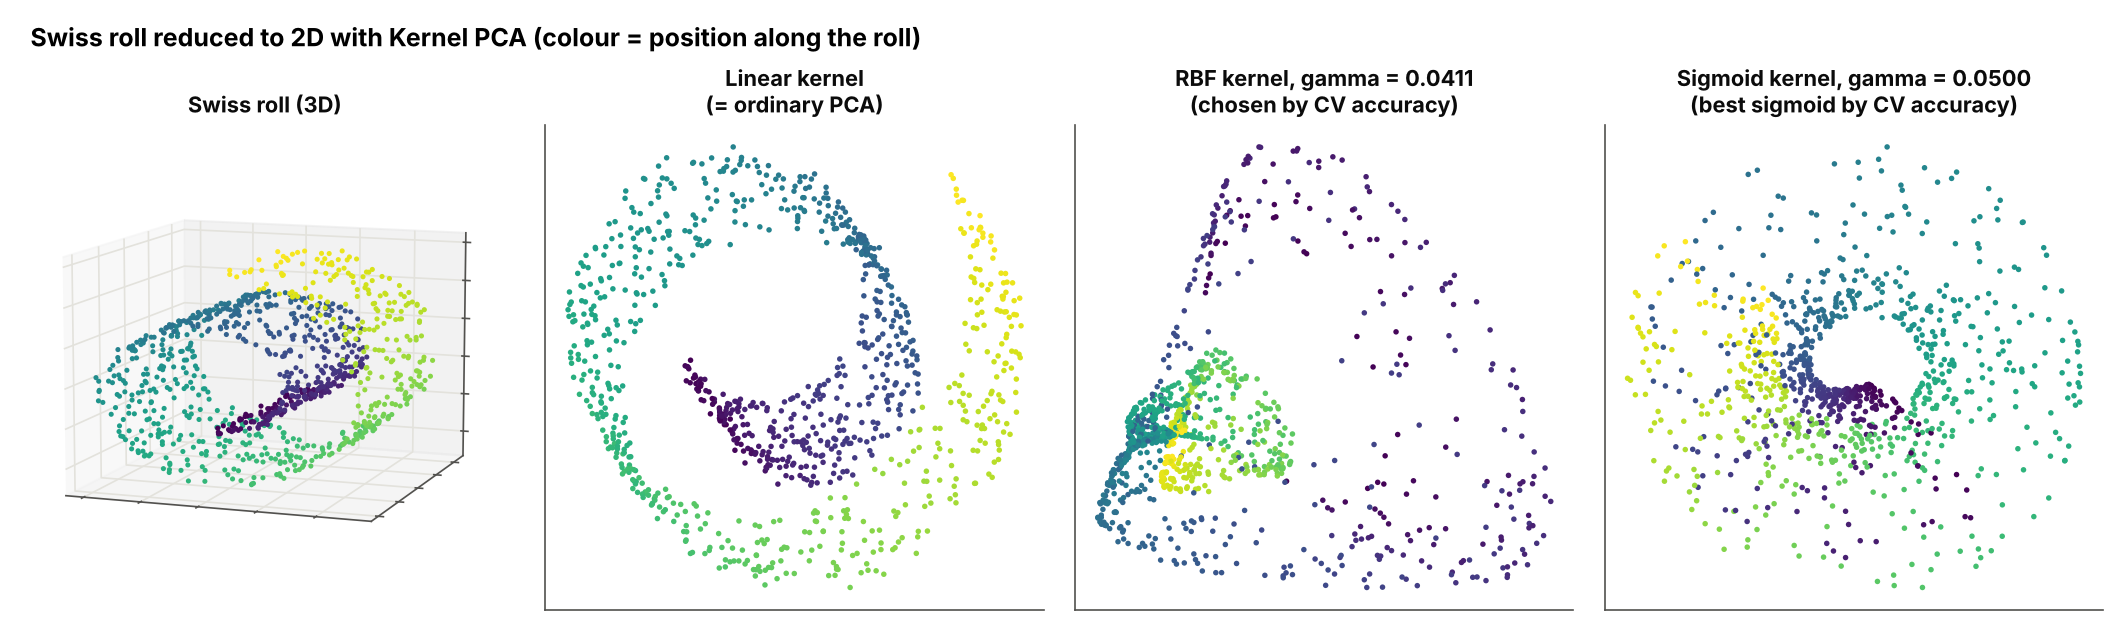
\includegraphics[width=\textwidth]{c_swiss_roll_kpca.png}
\caption{The Swiss roll and three Kernel PCA projections (colour = position $t$ along the roll).}
\label{fig:kpca}
\end{figure}

\begin{figure}[H]
\centering
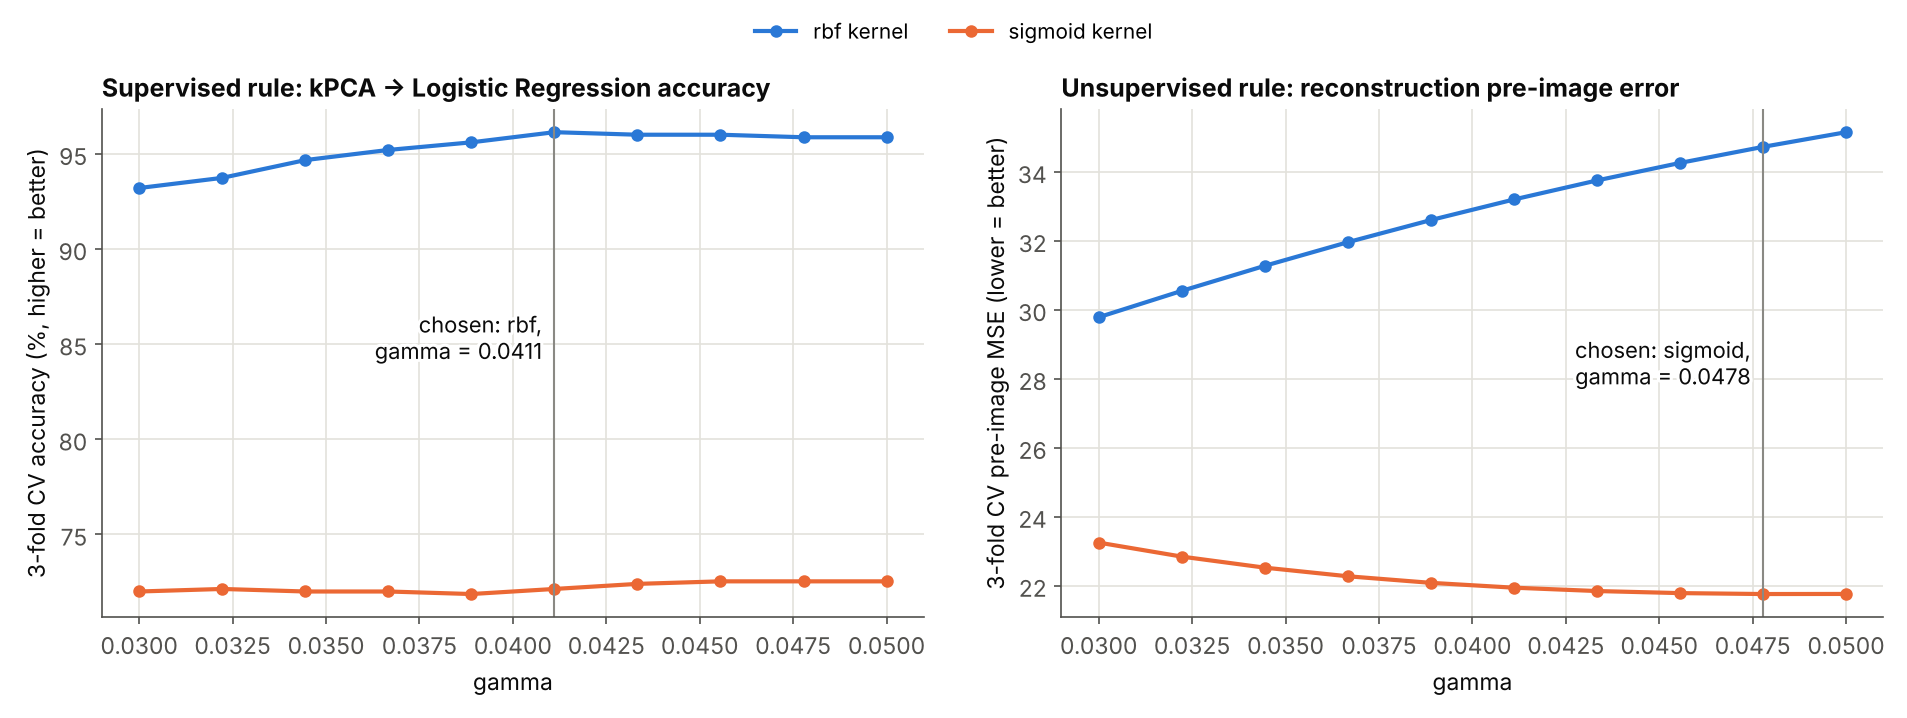
\includegraphics[width=\textwidth]{c_kpca_selection.png}
\caption{Left: supervised selection by cross-validated accuracy. Right: unsupervised selection by held-out pre-image error. Each rule picks a different kernel.}
\label{fig:kpcasel}
\end{figure}

%=====================================================================================
\section{Manifold learning and 2D maps}\label{sec:manifold}

\subsection{Locally Linear Embedding}

LLE first reconstructs every point from its $k$ nearest neighbours (Equation~8-4) and then finds low-dimensional points that keep those reconstruction weights (Equation~8-5).

\emph{Step 1.} For one point $\x$ with neighbours $\bm{\eta}_1,\dots,\bm{\eta}_k$ and weights summing to one,
\begin{equation}
\Big\|\x-\sum_{j}w_j\bm{\eta}_j\Big\|^2=\Big\|\sum_j w_j(\x-\bm{\eta}_j)\Big\|^2=\sum_{j,l}w_jw_l\,G_{jl},\qquad G_{jl}=(\x-\bm{\eta}_j)\T(\x-\bm{\eta}_l),
\end{equation}
where we used $\sum_j w_j=1$ to move $\x$ inside the sum. Minimising $\w\T\mathbf{G}\w$ subject to $\mathbf{1}\T\w=1$ with a multiplier $\nu$ gives $2\mathbf{G}\w=\nu\mathbf{1}$. Hence $\w\propto\mathbf{G}^{-1}\mathbf{1}$, and the constraint fixes the scale:
\begin{equation}
\w=\frac{\mathbf{G}^{-1}\mathbf{1}}{\mathbf{1}\T\mathbf{G}^{-1}\mathbf{1}} .
\end{equation}
($\mathbf{G}$ is regularised when $k$ exceeds the dimension.)

\emph{Step 2.} With the weight matrix $\W$ fixed, write the cost of Equation~8-5 as $\sum_i\|\z^{(i)}-\sum_jw_{ij}\z^{(j)}\|^2=\|(\mathbf{I}-\W)\mathbf{Z}\|_F^2=\tr\!\big(\mathbf{Z}\T\mathbf{M}\mathbf{Z}\big)$ with $\mathbf{M}=(\mathbf{I}-\W)\T(\mathbf{I}-\W)$. To exclude the trivial solution $\mathbf{Z}=\mathbf{0}$, impose $\frac{1}{m}\mathbf{Z}\T\mathbf{Z}=\mathbf{I}$. The minimiser is then given by the eigenvectors of $\mathbf{M}$ with the smallest eigenvalues. The constant vector, with eigenvalue 0 because each row of $\W$ sums to one, is discarded.

\subsection{Isomap, MDS and t-SNE}

The book describes three more methods. Multidimensional Scaling (MDS) keeps the pairwise distances. Isomap keeps \emph{geodesic} distances along a nearest-neighbour graph. t-SNE keeps similar instances close and dissimilar ones apart, and is mostly used for visualisation. t-SNE and MDS have no \texttt{transform} method, so they can only place the points they were fitted on. This matters for the deployed service (Section~\ref{sec:system}).

\subsection{How good is a 2D map?}

Exercise~7 of the book answers this question: a reduction can be judged by the performance of the algorithm that uses it. On the Swiss roll, a standardised Logistic Regression is trained on the 2D coordinates to tell the two halves of the roll apart. On MNIST, a 5-nearest-neighbour classifier is trained on the 2D coordinates. In both cases the score is the cross-validated accuracy. A high score means that points of the same class form their own regions.

\subsection{Results}

On the Swiss roll (Table~\ref{tab:manifold}, Figure~\ref{fig:manifold}), Isomap (\R{C.isomap}\%), t-SNE (\R{C.tsne}\%) and LLE (\R{C.lle}\%) separate the two halves almost perfectly. PCA (\R{C.pca}\%) and MDS (\R{C.mds}\%) cannot, because they preserve straight-line distances across the layers of the roll. LLE's best axis follows the position along the roll almost exactly (correlation \R{C.lleCorr}), but the spacing is uneven, as the book notes.

\begin{table}[H]
\centering
\caption{Manifold methods on the Swiss roll.}
\label{tab:manifold}
\small\TableManifold
\end{table}

\begin{figure}[H]
\centering
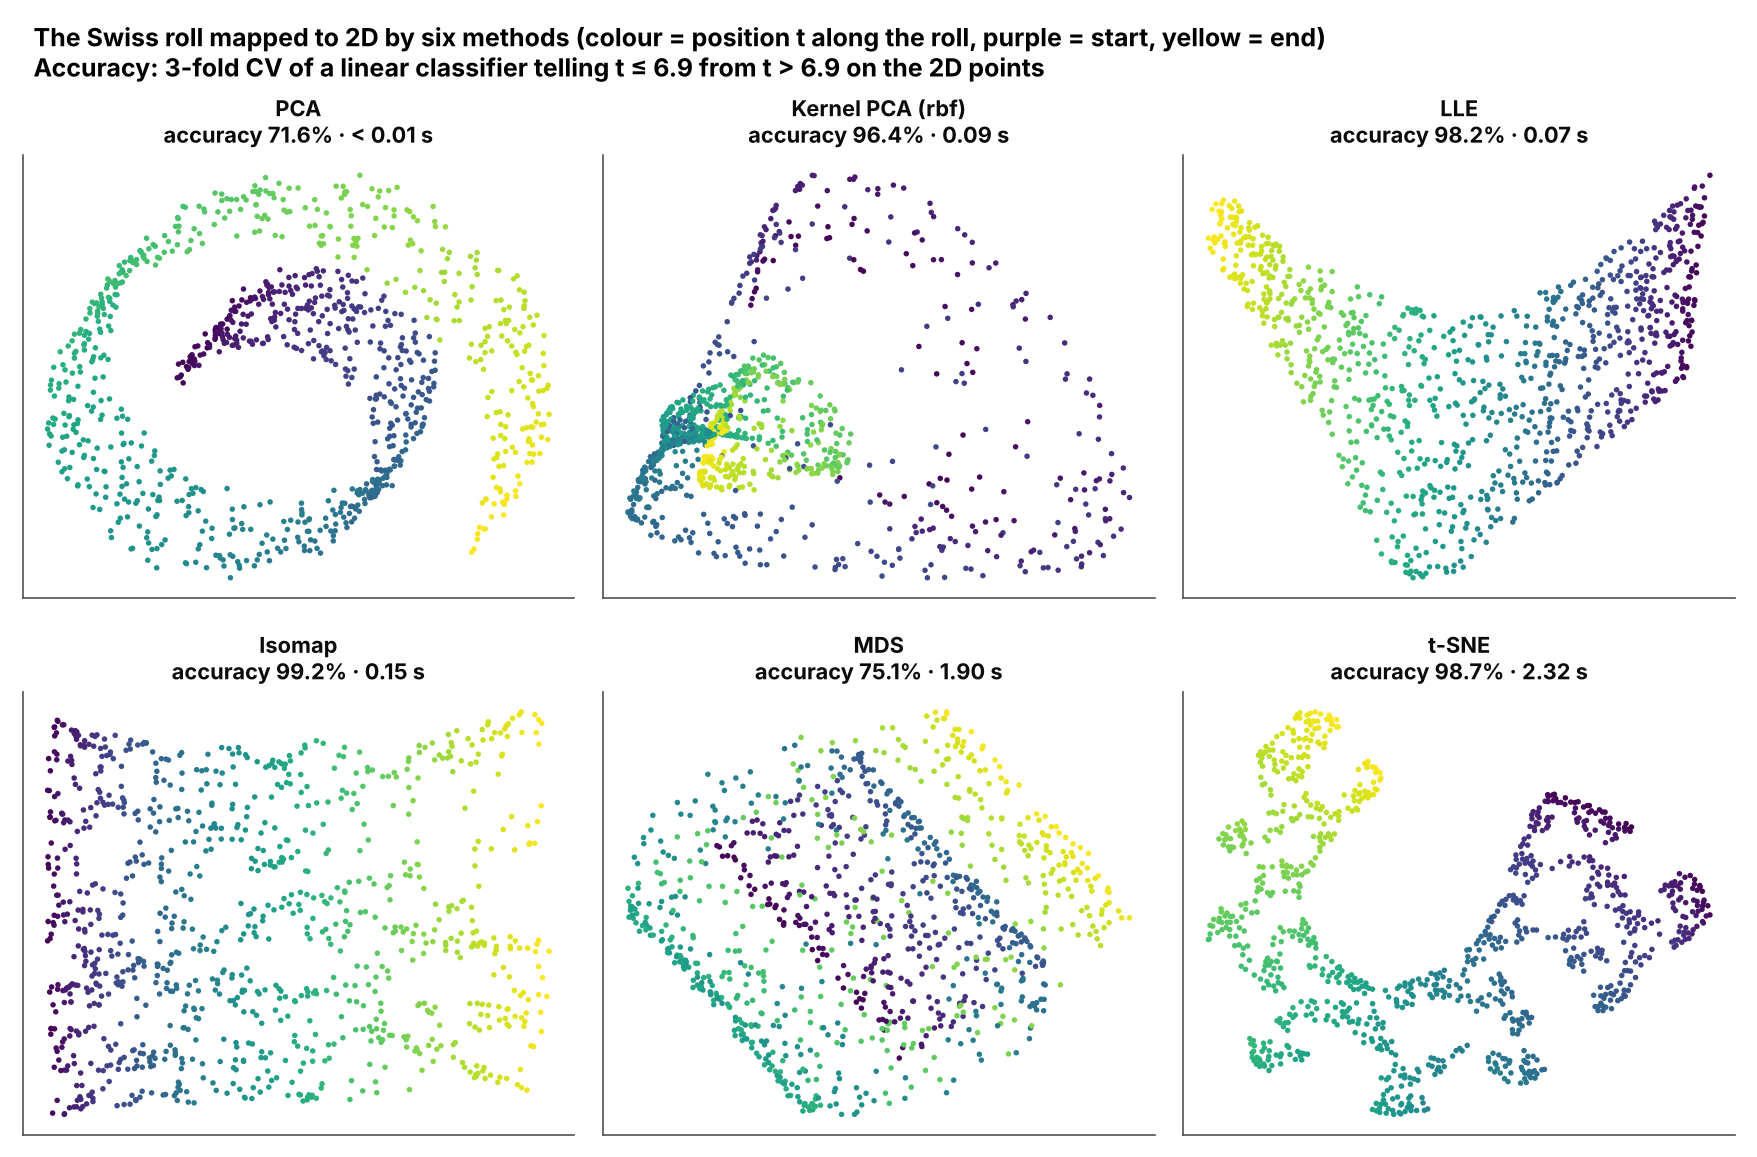
\includegraphics[width=0.9\textwidth]{c_manifold_methods.png}
\caption{The Swiss roll mapped to 2D by six methods.}
\label{fig:manifold}
\end{figure}

On MNIST (\R{D.n} training digits; Table~\ref{tab:maps} and Figures~\ref{fig:tsne} and~\ref{fig:maps}), t-SNE is in a class of its own, with \R{D.tsne}\% kNN accuracy in 2D. The next best is LLE with \R{D.lle}\%. PCA reaches \R{D.pca}\% and MDS \R{D.mds}\%, and MDS takes \R{D.mdssec}~s. The nonlinear methods run after a PCA that keeps 95\% of the variance, as in the book's exercise~8. The control run of t-SNE on the raw pixels shows that this chaining costs nothing: \R{D.tsneraw}\% in \R{D.tsnerawsec}~s, against \R{D.tsne}\% in \R{D.tsnesec}~s. For reference, the same classifier on all 784 pixels reaches \R{D.knn784}\% $\pm$ \R{D.knn784std}\% (standard deviation over the five folds), so in two numbers per image t-SNE separates the digits as well as the full pixel vectors do. This comparison flatters t-SNE a little. Because t-SNE and MDS cannot place new points, every map is fitted on all \R{D.n} points before the cross-validation, so the test folds have already shaped the layout. The score therefore describes how well a map separates the digits; it is not a held-out classification accuracy.

\begin{table}[H]
\centering
\caption{2D maps of \R{D.n} MNIST training digits.}
\label{tab:maps}
\small\TableMaps
\end{table}

\begin{figure}[H]
\centering
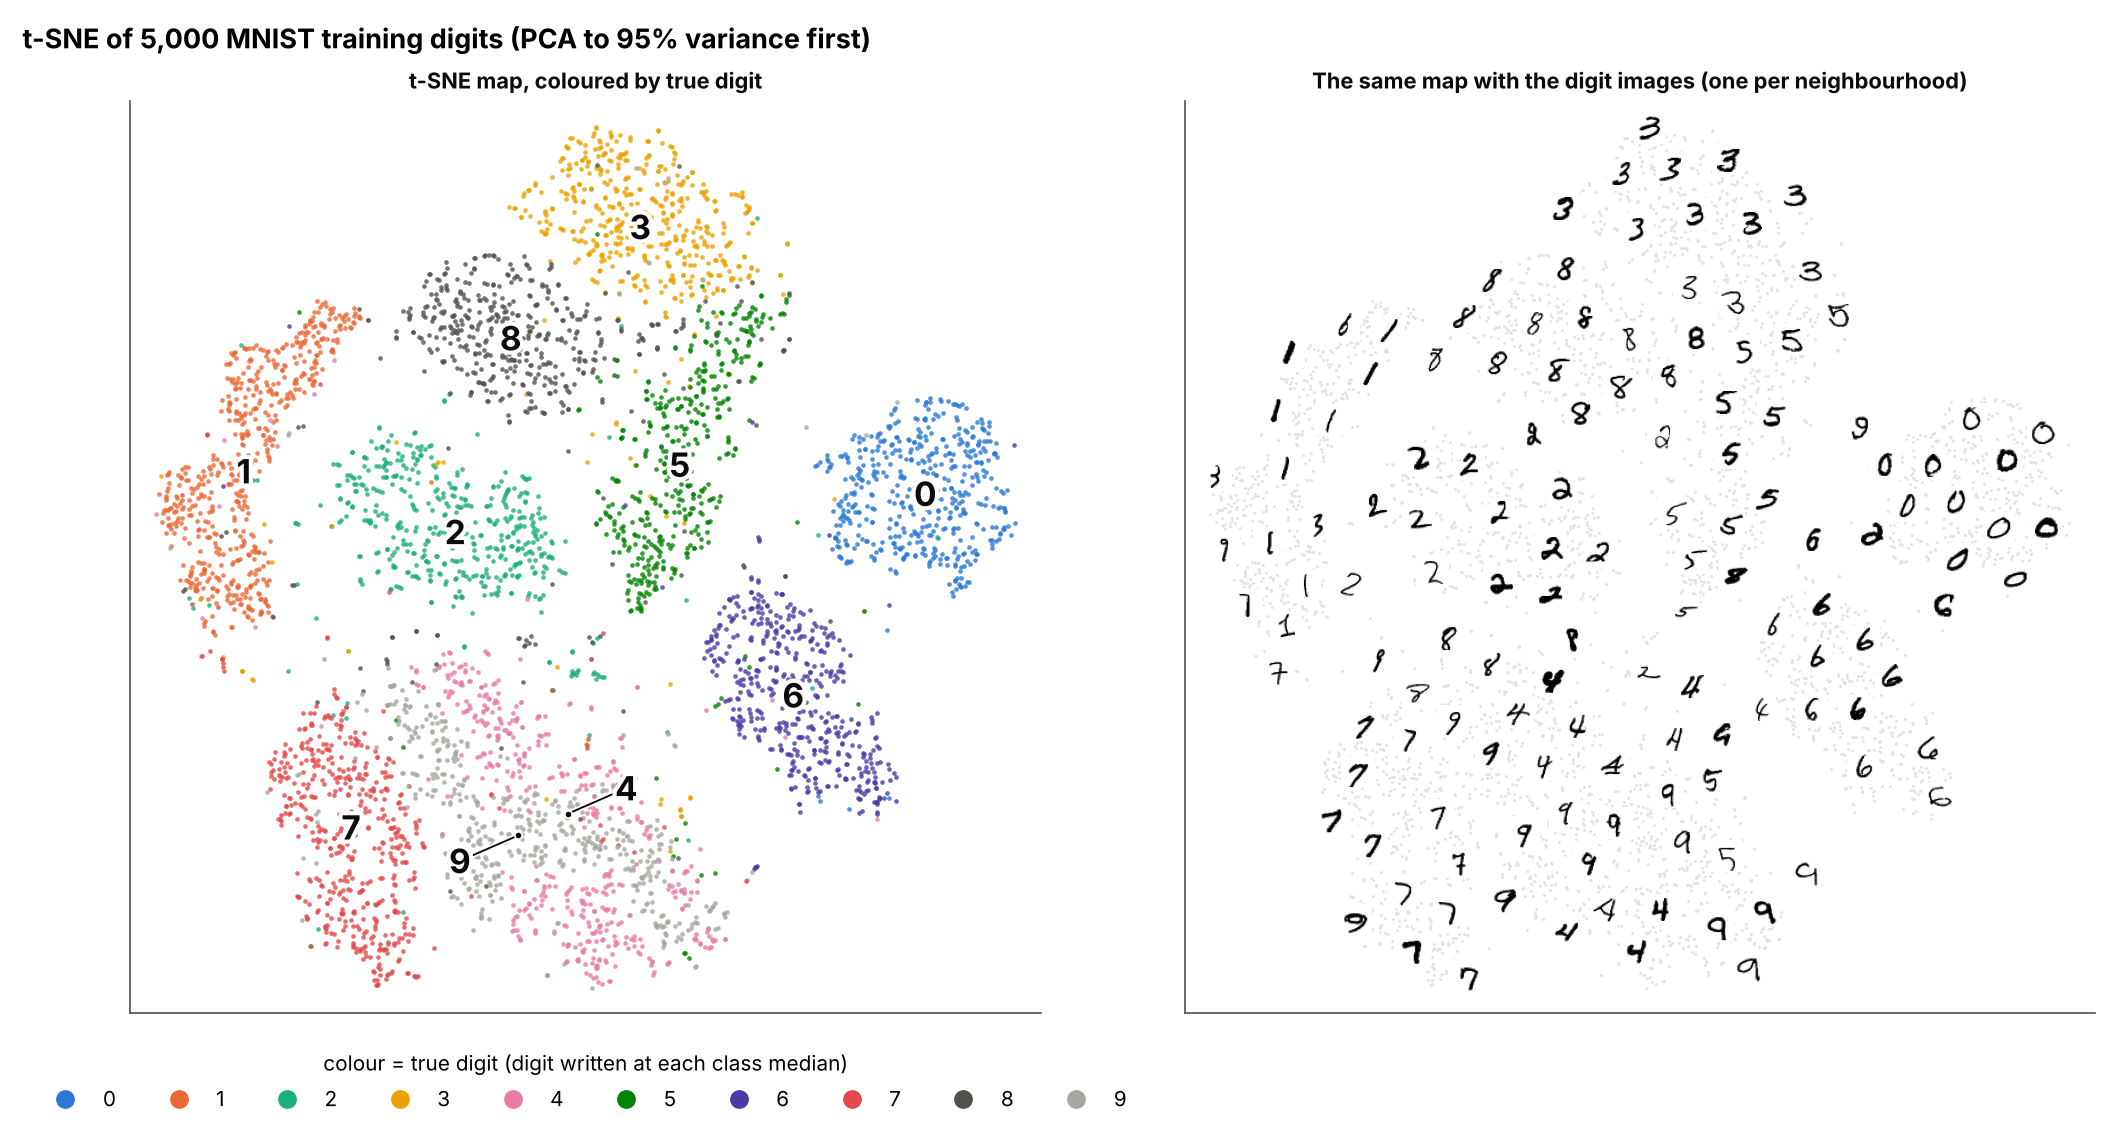
\includegraphics[width=\textwidth]{d_tsne_map.png}
\caption{t-SNE map of MNIST. Right: one digit image wherever no other image is already close (the book's suggestion in exercise~10).}
\label{fig:tsne}
\end{figure}

\begin{figure}[H]
\centering
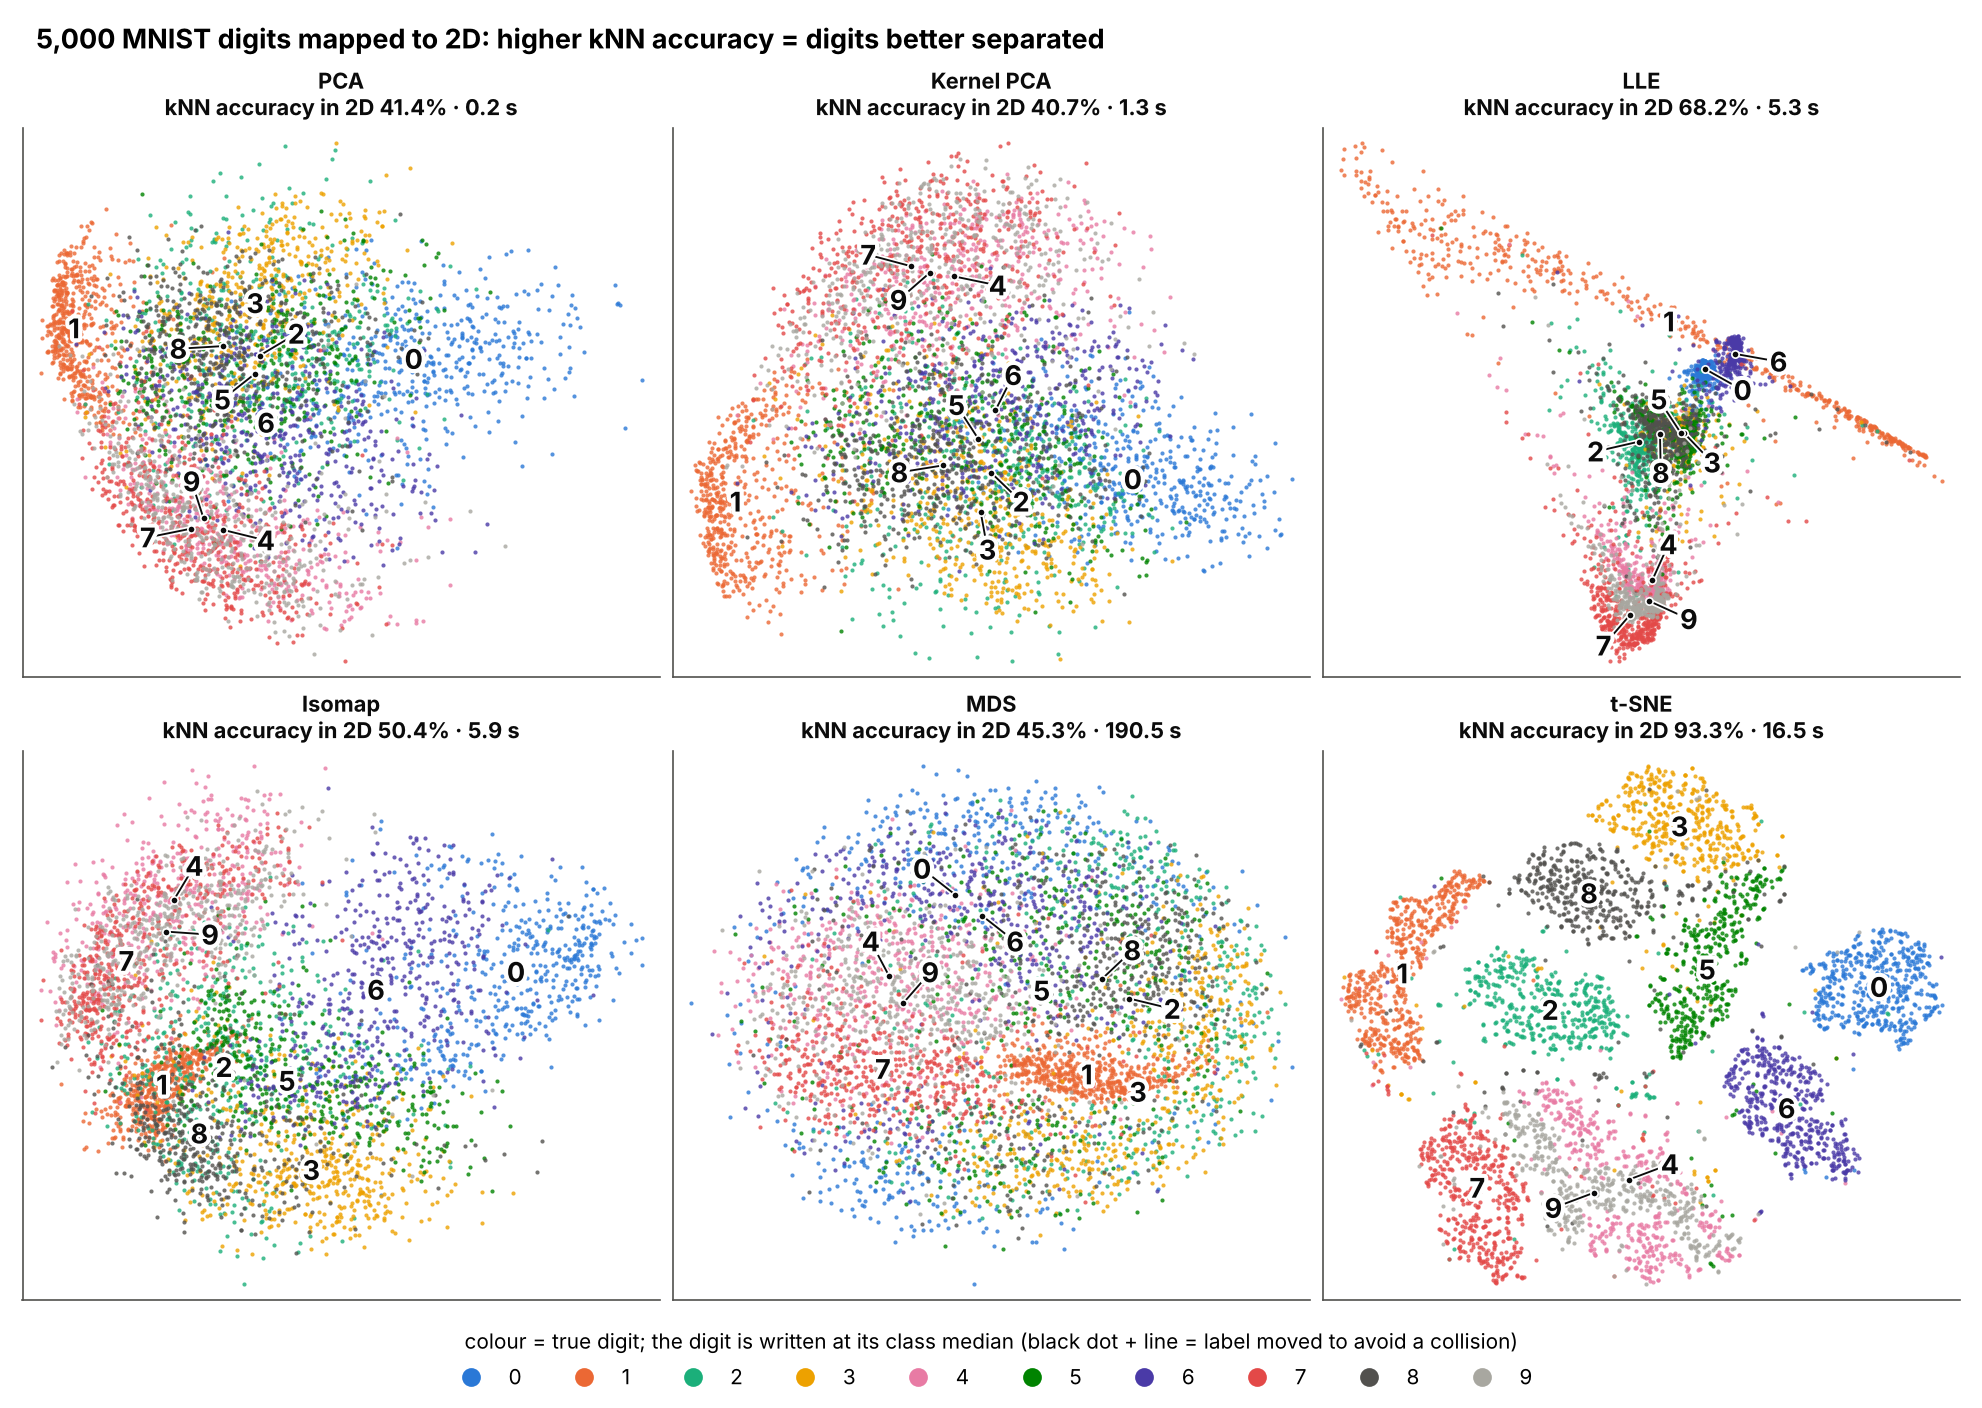
\includegraphics[width=\textwidth]{d_maps_comparison.png}
\caption{The same digits mapped by six methods.}
\label{fig:maps}
\end{figure}

%=====================================================================================
\section{Compressed features for classification}\label{sec:classify}

Exercise~9 of the book trains a Random Forest on the raw pixels and on the PCA features, and compares training time and accuracy. The same comparison is run for Softmax Regression and for an RBF-kernel SVM, the classifier the book says PCA can speed up ``tremendously''. The SVM is trained on \R{E.svmn} random training images, because kernel SVMs scale roughly quadratically with the number of samples. The PCA is unsupervised, so it is fitted on all 60{,}000 training images (\R{E.svmd} components, the same as in Section~\ref{sec:pca}), and its fit time is included in the training time. Both SVMs use scikit-learn's defaults, $C=1$ and \texttt{gamma="scale"}; neither is tuned. Table~\ref{tab:clf} and Figure~\ref{fig:clf} give the results.

\begin{table}[H]
\centering
\caption{Classifiers on raw pixels and on PCA features (95\% of the variance), evaluated on the 10{,}000 test images.}
\label{tab:clf}
\small\TableClassifiers
\end{table}

\begin{figure}[H]
\centering
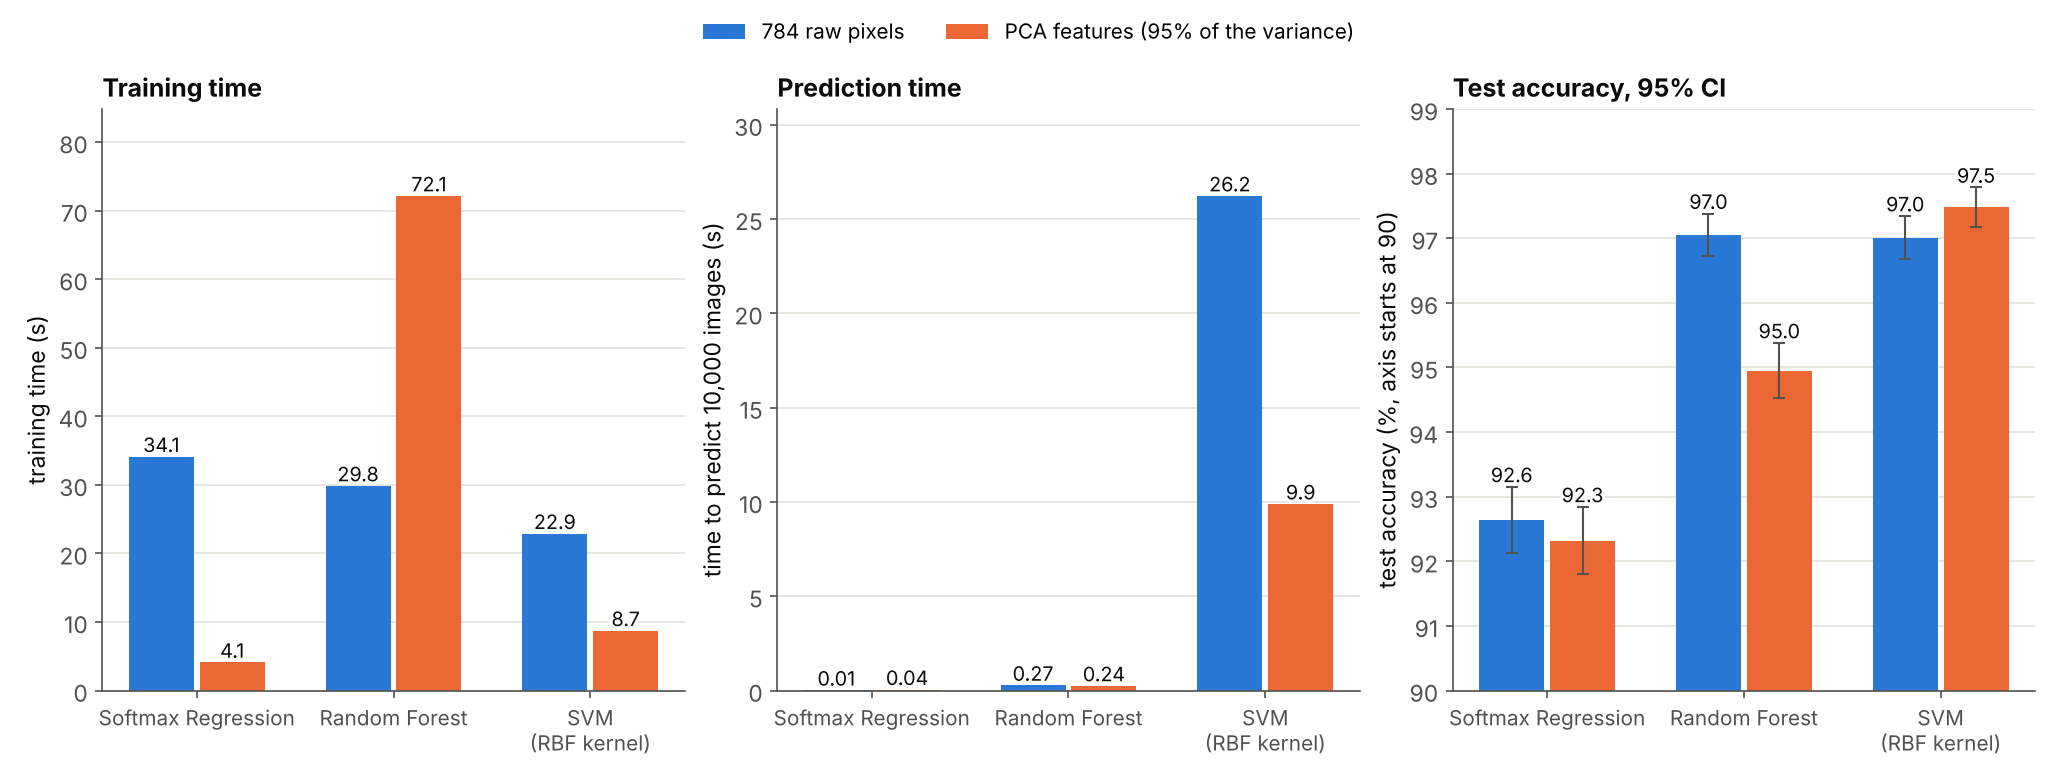
\includegraphics[width=\textwidth]{e_classification.png}
\caption{Training time, prediction time and accuracy with and without PCA.}
\label{fig:clf}
\end{figure}

\begin{itemize}
\item \textbf{SVM.} PCA makes training \R{E.svmfit} times and prediction \R{E.svmpred} times faster. Evaluating an RBF kernel costs $O(n)$ per pair of points, so cutting $n$ from 784 to \R{E.svmd} cuts the cost of every kernel evaluation. The stored model also shrinks, from \R{E.svmrawMB}~MB to \R{E.svmpcaMB}~MB, because each support vector is now stored as \R{E.svmd} numbers instead of 784. Accuracy changes from \R{E.svmraw}\% to \R{E.svmpca}\%, a difference of \R{E.svmdiff}~pp with a paired 95\% interval of \R{E.svmdifflo} to \R{E.svmdiffhi}~pp.

The accuracy change has a second cause besides the compression. \texttt{gamma="scale"} sets $\gamma=1/(n\,\mathrm{Var}(\X))$, which gives a different kernel width on the PCA features than on the pixels. An ablation therefore runs the PCA SVM with the raw model's $\gamma$. Since PCA nearly preserves the distances between images, the two models then use almost the same kernel. This variant scores \R{E.same}\%, \R{E.samediff}~pp against raw pixels (95\% interval \R{E.samedifflo} to \R{E.samediffhi}~pp). Of the \R{E.svmgain}~pp gain, only \R{E.samegain}~pp therefore remains when the kernel width is held fixed, and the lower end of its interval is close to zero. Most of the accuracy gain comes from the different bandwidth that \texttt{gamma="scale"} chooses on the PCA features. The speed-up, in contrast, is a property of PCA itself. Tuning $\gamma$ for each representation would be the fair next comparison.
\item \textbf{Softmax Regression.} Training is \R{E.smfit} times faster, and accuracy changes by \R{E.smdiff}~pp (95\% interval \R{E.smdifflo} to \R{E.smdiffhi}~pp).
\item \textbf{Random Forest.} Training is \emph{slower} with PCA (\R{E.rfpcasec}~s against \R{E.rfrawsec}~s), and accuracy drops from \R{E.rfraw}\% to \R{E.rfpca}\% (\R{E.rfdiff}~pp, 95\% interval \R{E.rfdifflo} to \R{E.rfdiffhi}~pp), as the book's exercise warns. The stored forest also grows from \R{E.rfrawMB}~MB to \R{E.rfpcaMB}~MB, so its trees have many more nodes. A plausible explanation, not isolated here, is that each principal component mixes all pixels: a single split on it separates the classes less cleanly than a split on one well-placed pixel, so the trees need more splits.
\end{itemize}
Whether compression helps therefore depends on the model that comes after it. This is why the deployed pair is the SVM, and why the API serves both models side by side.

%=====================================================================================
\section{Flagging unusual inputs with the reconstruction error}\label{sec:detector}

\subsection{Score and threshold}

The detector combines two ideas from the book. The first is the PCA reconstruction error of Chapter~8: an input is scored by
\begin{equation}
e(\x)=\frac{1}{n}\big\|\x-\hat{\x}\big\|^2=\frac{1}{n}\big\|(\mathbf{I}-\W_d\W_d\T)(\x-\bmu)\big\|^2 .
\end{equation}
Digits resemble the training data and are rebuilt well; inputs unlike them are not. The second is the percentile rule of Chapter~9 (p.~266): flag the 4\% worst-scoring instances. The PCA ($d=\R{F.d}$) is fitted on 50{,}000 training images. The threshold $\tau$ is the 96th percentile of $e$ on the other 10{,}000 training images, $\tau=\R{F.thr}$. If new clean digits come from the same distribution as these held-out images, the probability that one exceeds $\tau$ is 4\%, up to a correction of order $1/10{,}000$. A threshold set on the fitting images ($\tau=\R{F.trainthr}$) would be optimistic in general. With 50{,}000 images, however, PCA hardly overfits and both thresholds give similar rates: \R{F.fa}\% (95\% interval \R{F.falo}--\R{F.fahi}\%) and \R{F.fatrain}\% false alarms on the test digits. Both are below 4\% because MNIST's test digits are rebuilt slightly better than its training digits (Table~\ref{tab:variance}).

\subsection{Results and blind spots}

Each test image is corrupted in eight ways (Table~\ref{tab:detector}, Figures~\ref{fig:hist} and~\ref{fig:examples}). Random noise, inverted, shuffled and Gaussian-noise images are all flagged, and \R{F.shifted}\% of the shifted ones. Upside-down (\R{F.rotated}\%) and mirrored (\R{F.mirrored}\%) digits are mostly missed: they are still made of digit-like strokes, which the components can rebuild. Dimmed digits are never flagged (\R{F.dimmed}\%). The reason follows from the score. For $\tilde\x=\alpha\x$ with $0<\alpha<1$,
\begin{equation}
(\mathbf{I}-\W_d\W_d\T)(\alpha\x-\bmu)=\alpha\,(\mathbf{I}-\W_d\W_d\T)(\x-\bmu)-(1-\alpha)\,(\mathbf{I}-\W_d\W_d\T)\,\bmu .
\end{equation}
When the mean image is itself well rebuilt, the second term is small and $e(\alpha\x)\approx\alpha^2e(\x)$. For $\alpha=0.3$ this predicts a 91\% \emph{smaller} error. The measured median falls from 198 to 18, in agreement. A low-intensity input looks \emph{more} normal to this score, so a second, lower threshold or an intensity check would be needed to catch it.

Over the eight corruptions the mean detection rate is \R{F.mean}\%, and the ROC-AUC between clean and corrupted inputs is \R{F.auc}. These two averages depend on which corruptions are included, so the per-type rates are the informative numbers. All of them are synthetic; no real out-of-distribution images (letters, other datasets) were tested. The 4\% target is the book's rule of thumb, not a choice derived from the cost of a false alarm. A detector with fewer components separates them slightly better: \R{F.bestvar}\% of the variance ($d=\R{F.bestvard}$) gives an AUC of \R{F.bestvarAUC} (Table~\ref{tab:varsweep}). The deployed SVM is wrong on \R{F.errflag}\% of the \R{F.nflag} clean test digits that are flagged, and on \R{F.errunflag}\% of the rest. The flag therefore marks harder inputs, but it catches only \R{F.nerrflag} of the classifier's \R{F.nerr} errors. It is a guard against inputs that are not digits, not an estimate of the classifier's confidence.

\begin{table}[H]
\centering
\caption{Flag rate at the deployed threshold.}
\label{tab:detector}
\small\TableDetector
\end{table}

\begin{table}[H]
\centering
\caption{Detector quality against the number of components.}
\label{tab:varsweep}
\small\TableVarSweep
\end{table}

\begin{figure}[H]
\centering
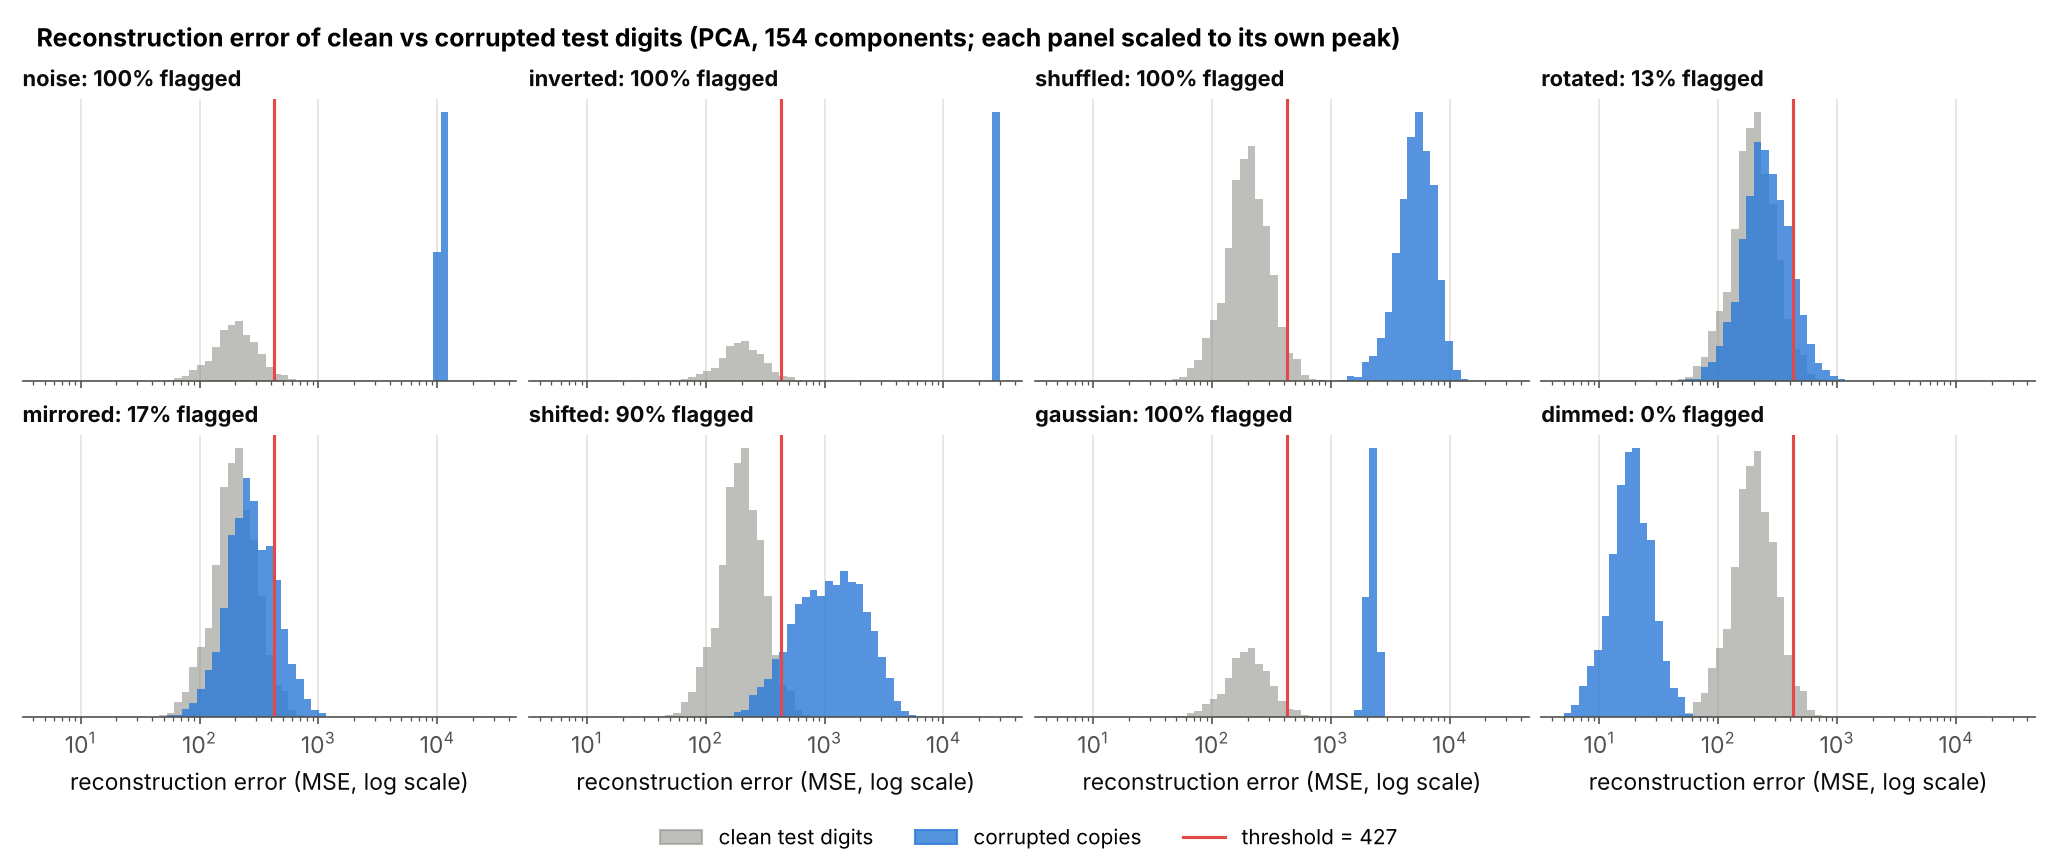
\includegraphics[width=\textwidth]{f_error_histograms.png}
\caption{Reconstruction errors of clean and corrupted test digits, with the threshold.}
\label{fig:hist}
\end{figure}

\begin{figure}[H]
\centering
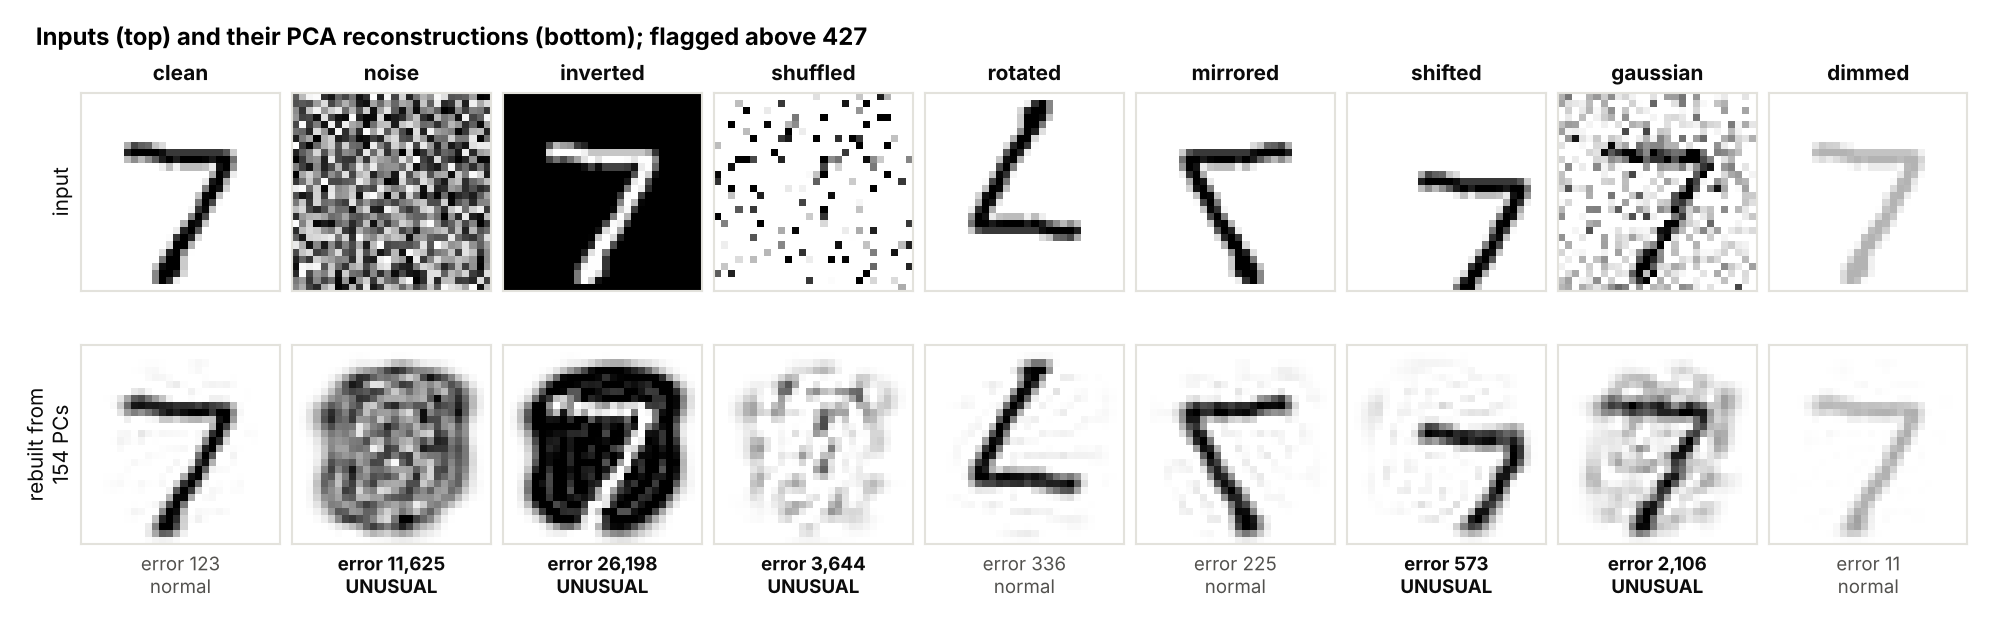
\includegraphics[width=\textwidth]{f_corruption_examples.png}
\caption{One test digit, its corruptions and their reconstructions from 154 components.}
\label{fig:examples}
\end{figure}

%=====================================================================================
\section{From notebook to service}\label{sec:system}

\begin{figure}[H]
\centering
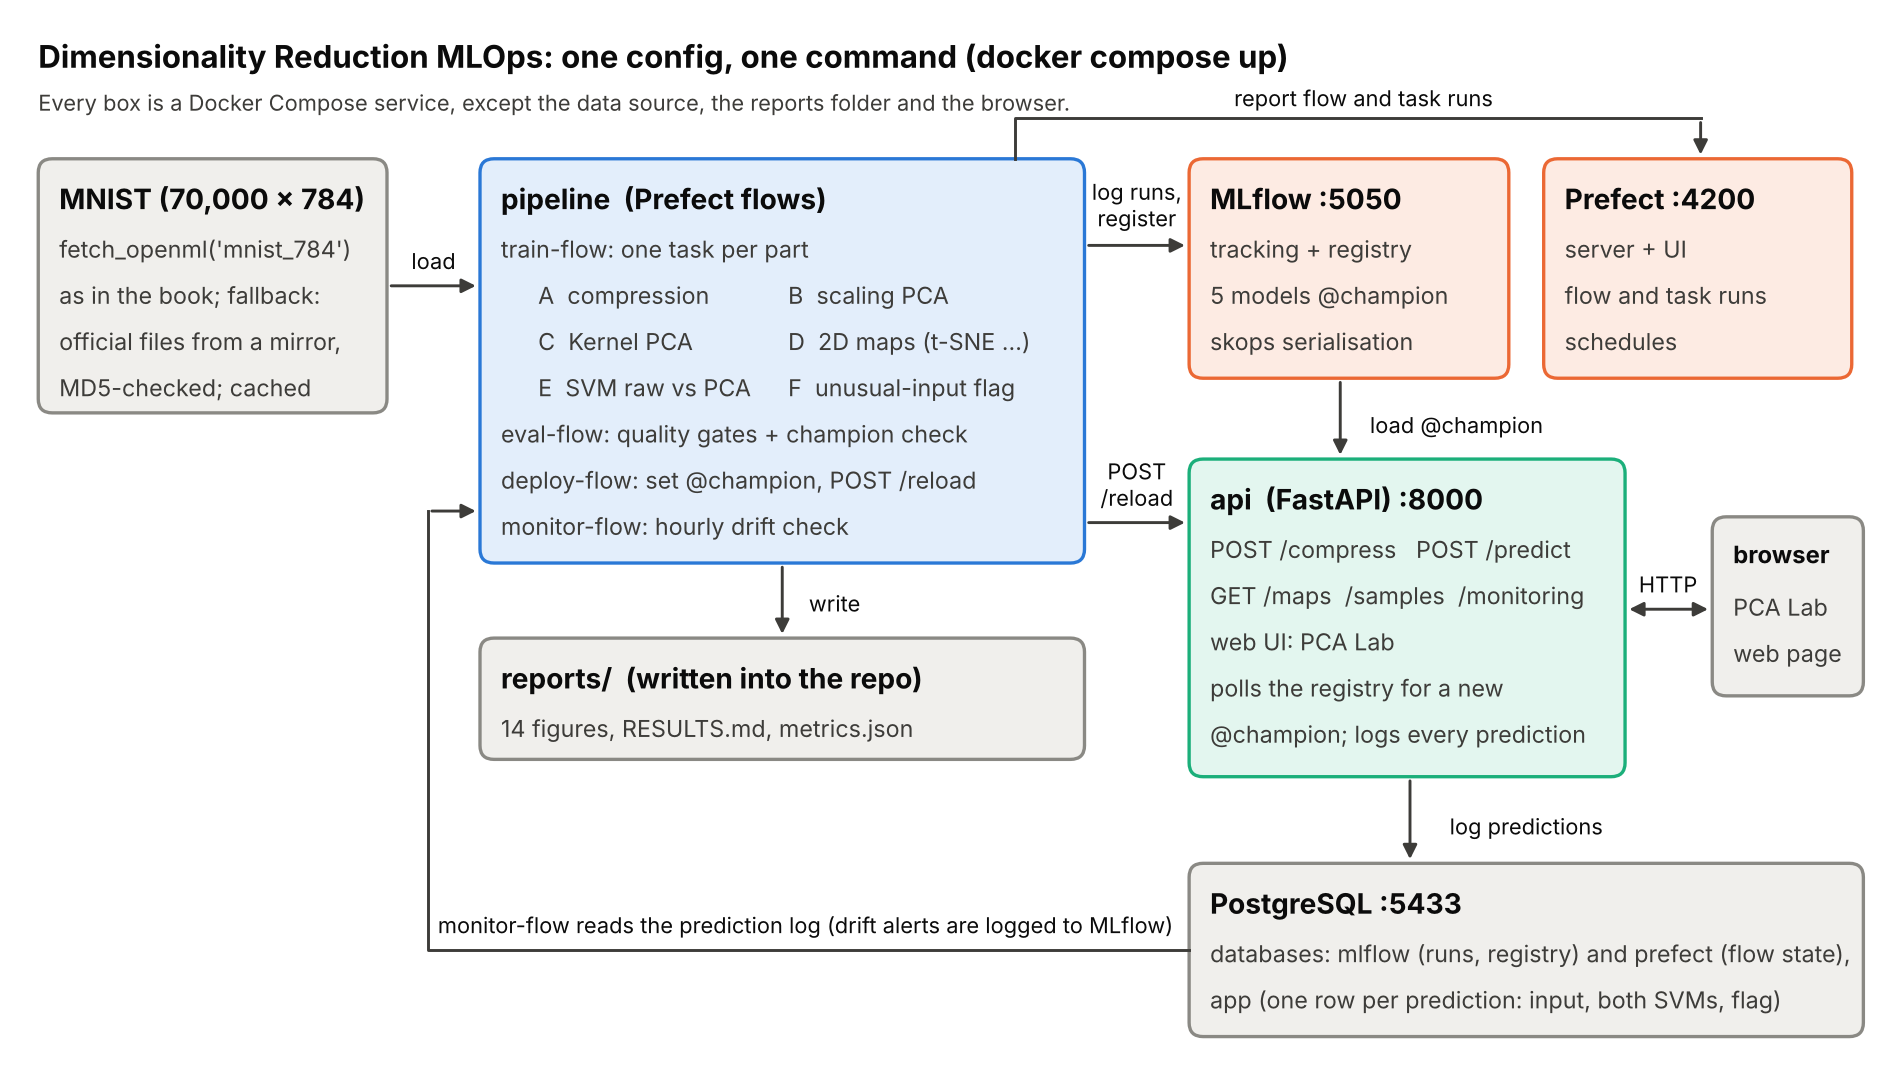
\includegraphics[width=\textwidth]{architecture.png}
\caption{System architecture. All services start with \texttt{docker compose up}.}
\label{fig:arch}
\end{figure}

The experiments are packaged as a small production system (Figure~\ref{fig:arch}). It follows the structure of a full-stack on-premises MLOps reference project, reduced to the parts this problem needs.

\paragraph{One configuration, one command.} A YAML file describes the data split, every experiment, the quality gates and the deployment target. The command
\begin{center}\texttt{python run\_flow.py --config configs/full\_flow\_config.yaml}\end{center}
runs train $\to$ evaluate $\to$ deploy as Prefect flows. Inside Docker Compose the same command runs in the \texttt{pipeline} container. A quick configuration trains on a 10{,}000-image subset for continuous integration.

\paragraph{Tracking and registry.} Each part (A--F) logs its parameters, metrics, tables and figures to its own nested MLflow run. Five models are registered with skops serialisation instead of pickle: the full PCA used for compression, the two SVMs, the reconstruction-error detector, and an \emph{embedding atlas}. Before loading a model, the code checks that it asks to trust no custom types beyond an allow-list kept in the code itself. The atlas holds 2{,}000 points of every 2D map together with the fitted PCA, Kernel PCA and LLE reducers that can place new inputs.

\paragraph{Quality gates.} The evaluation flow reloads the registered models and re-measures them on the test set. A candidate is promoted to the \texttt{@champion} alias only if every check passes:
\begin{itemize}
\item at most 200 components for 95\% of the variance, and at least 94\% of the test variance kept;
\item both classifiers at least 95\% accurate, with the PCA classifier at most 1~pp behind the raw-pixel classifier;
\item at most 6\% false alarms on clean digits, and at least 95\% detection of noise, inverted and shuffled inputs;
\item at least three maps able to place new points;
\item no classifier more than 0.5~pp worse than the current champion.
\end{itemize}

\paragraph{Serving and monitoring.} A FastAPI service loads the champions and offers several endpoints. \texttt{/compress} keeps any number of components and returns the rebuilt image. \texttt{/predict} returns both SVMs, the unusual-input flag and the input's position on the maps. \texttt{/maps} and \texttt{/samples} feed the web interface. The service polls the registry for a new champion and logs every prediction to PostgreSQL. A scheduled monitoring flow raises an alert when the share of unusual inputs exceeds three times the expected 4\%, when one digit dominates the predictions, or when the two classifiers disagree too often.

\paragraph{Operations.} The pipeline exits with a non-zero code when a gate fails, and checks at start-up that it can write its reports. If the service cannot load a newly promoted set of models, the deploy flow restores the previous champion. The API loads each model by its resolved version number and ignores a half-finished promotion, so it never serves a mixed set. Every registered version is tagged with the MD5 of the data, the hash of the configuration and the git commit. Database passwords are removed from the configuration before it is logged. The scheduled drift check ignores demo and CI traffic.

\paragraph{Testing.} pytest covers the data checks (including the MD5 rejection of a wrong file), the mathematical identities above, every experiment on small data, the gates, the monitoring rules and the API. An integration test runs the full Prefect and MLflow flow on an MNIST subset. GitHub Actions runs linting and the tests on Python 3.12 and 3.13, then builds the Docker images and smoke-tests the deployed service.

%=====================================================================================
\section{Limitations and next steps}

\begin{itemize}
\item MNIST has a fixed split, so the results come from one test set of 10{,}000 images, given with confidence intervals. The same test set also drives the quality gates and the threshold sweep; a separate validation split would keep it untouched until the final report. Timings depend on the machine.
\item The SVMs use default hyperparameters. Tuning $C$ and $\gamma$ for each representation, and an accuracy-versus-$d$ curve, would separate the effect of compression from that of the kernel width more fully than the ablation above.
\item The SVM is trained on \R{E.svmn} images to keep the pipeline fast. Training on all 60{,}000 would raise accuracy at a higher cost.
\item The detector misses dimmed, mirrored and upside-down digits, and was tested on synthetic corruptions only. An intensity check, or a second score from a different model, would cover the first; real out-of-distribution images would test it properly.
\item t-SNE was run with one perplexity (30) and one seed. Its map is a visual summary, not a model that can place new inputs.
\item The deployed Kernel PCA uses scikit-learn's default $\gamma$ on MNIST. Tuning it for the maps, as was done on the Swiss roll, is a natural extension.
\item Only methods from Chapter~8 of the book are used. Autoencoders, a neural approach to the same problem, are covered later in the book.
\end{itemize}

\appendix
\section{Reproducing the results}

\begin{itemize}
\item Full stack: \texttt{docker compose up --build}, then open \url{http://localhost:8000}.
\item Local: \texttt{make install}, then \texttt{make train} (all 70{,}000 images) or \texttt{make quick}.
\item Report: \texttt{python make\_numbers.py}, then \texttt{pdflatex technical\_report.tex} twice. Every number in this report is read from \texttt{reports/metrics.json}.
\end{itemize}

\end{document}
